%-------------------------------
% 4YP REPORT
%-------------------------------

% JAMES ROUTLEY

% COMPILE WITH XeLaTeX

%-------------------------------
% Preamble
%-------------------------------
\documentclass[11pt, a4paper]{report}
\linespread{1.72} % similar to double line spacing in word
\usepackage[margin=22mm]{geometry}
\usepackage{fontspec, amsmath, url}
\usepackage[hang,small]{caption} % make captions look better
\usepackage{url, hyperref}
\usepackage[backend=bibtex]{biblatex}
\bibliography{4yp}
\setmainfont{Arial}
\setlength{\parindent}{0in}
\setlength{\parskip}{0.5cm}
\newcommand{\HRule}{\rule{\linewidth}{0.5mm}}
\newcommand{\vect}[1]{\boldsymbol{#1}}
\usepackage[multiple]{footmisc} % puts a comma between multiple footnotes at one point
\usepackage{pdfpages}


%-------------------------------
% Document
%-------------------------------
\begin{document}




%-------------------------------
% Title
%-------------------------------
\begin{titlepage}
\begin{center}

% Upper part of the page. The '~' is needed because \\
% only works if a paragraph has started.

\includegraphics[width=0.16\textwidth]{img/OxfLogo.png}~\\[1.5cm]

\textsc{\LARGE University of Oxford}\\[1.5cm]
\textsc{\Large Fourth year project}\\[0.5cm]

% Title
\HRule \\[0.4cm]
{ \huge \bfseries A Flower Classification Application \\[0.4cm] }

\HRule \\[1.5cm]

% Author and supervisor
\noindent
\begin{minipage}[t]{0.4\textwidth}
\begin{flushleft} \large
\emph{Author:}\\
James \textsc{Routley} \\
Trinity College
\end{flushleft}
\end{minipage}%
\begin{minipage}[t]{0.4\textwidth}
\begin{flushright} \large
\emph{Supervisors:} \\
Professor~Andrew \textsc{Zisserman} \\
Dr Yuning \textsc{Chai}
\end{flushright}
\end{minipage}

\vfill

% Bottom of the page
{\large May 2015}

\end{center}
\end{titlepage}



\begin{abstract}
This project makes use of computer vision techniques to build a mobile application which performs image classification of flowers. The application can classify 102 flower species common to the United Kingdom, with a practical accuracy of 96.2\%.

The classification pipeline consists of feature extraction and followed by classification. An image of a flower is passed to a convolutional neural network which outputs a vector that describes the features of the flower. The dot products of the feature vector and 102 one-vs-the-rest support vector machine classifiers are found, giving 102 prediction values, which give the likelihood of the flower being each of those 102 flower species. These prediction values are then sorted, producing a ranked list of the flower’s most likely species. 

This classification pipeline is run on a server and is accessible from an application which is running on a user’s Android mobile device. The application allows the user to choose whether to take a photo of a flower or upload a previously captured flower image. This image is automatically uploaded to the classification pipeline, classified, and a list of the six highest predicted species are returned to the device. Images of these six flowers are displayed in a scrollable list on the device. If one of the images is clicked, a new screen comes up, displaying more information about that flower.
\end{abstract}






%-------------------------------
% Contents
%-------------------------------
\setlength{\parskip}{0.0cm}
\tableofcontents
\setlength{\parskip}{0.4cm}


%-------------------------------
% Introduction
%-------------------------------
\chapter{Introduction}

\section{Motivation}  

Classifying flower species is difficult for humans to do as it requires access to in-depth specialist knowledge; some flower species look similar, whilst other flowers look different despite being the same species, as shown in Figure~\ref{img:33}. Intuitively, the flower species classification accuracy of a non-expert human would be low, and to learn to differentiate between flower species would require a large time commitment.

\begin{figure}[hbt]
	\centering
  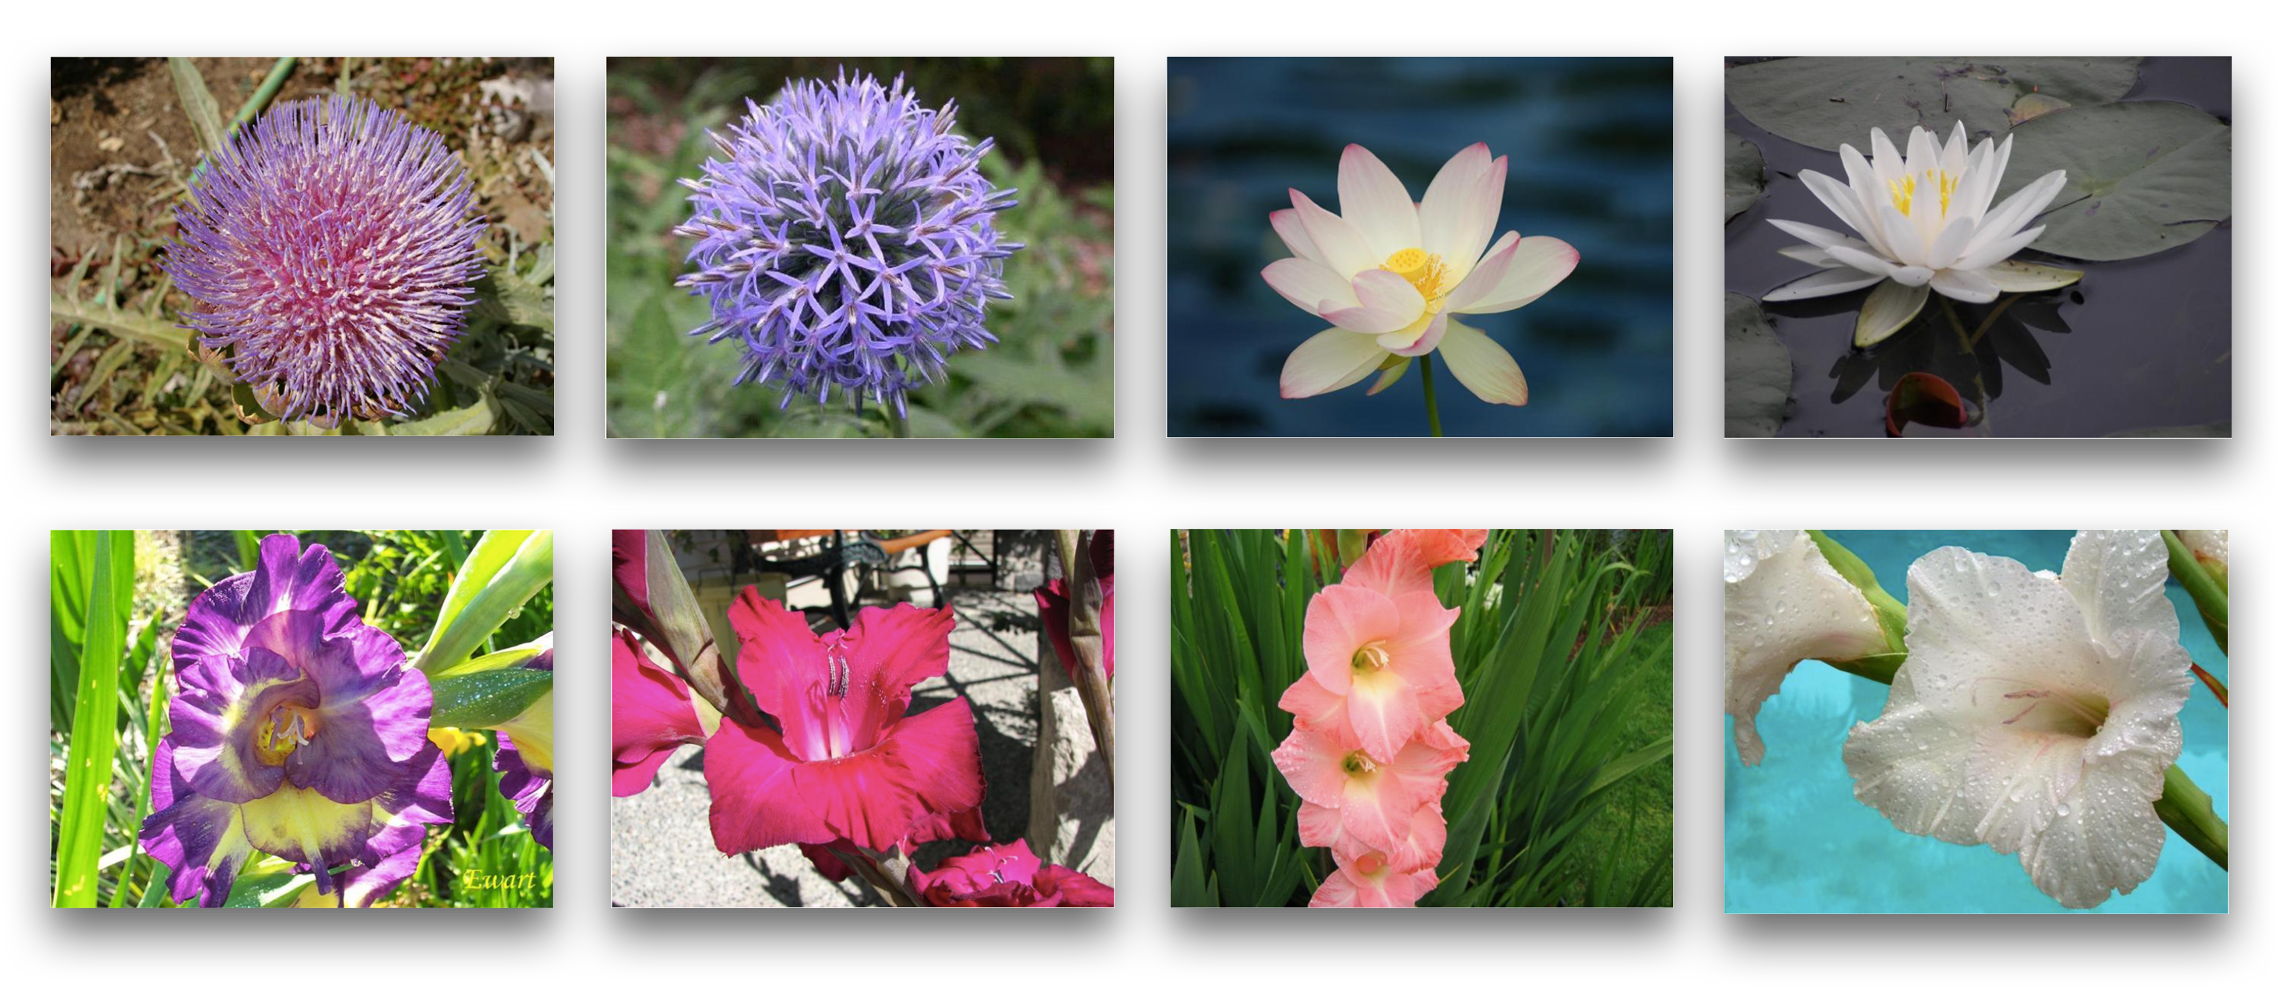
\includegraphics[totalheight=5cm]{img/33.png}
  \caption{Top row: different species which look similar (l-r: artichoke, globe thistle, lotus, water lily). Bottom row: difference within a species; all are examples of the sword lily.}
  \label{img:33}
\end{figure}

Currently, the standard method for classifying flowers is manual searching through lengthy field guides. Although tools like decision trees and digitalisation make the process easier, classification is still difficult for amateurs who may not possess the vocabulary to accurately describe the flower in question. 

This report presents an application which greatly simplifies this process, shown in Figure~\ref{img:47}. From a single photo of a flower, computer vision and machine learning algorithms are used to classify that flower’s species. The process is quick (in the order of seconds and has a practical accuracy of 96.2\%. It requires the user to have no prior knowledge and is robust to variations in photo quality, light levels and background content. No comparable applications are currently available. 

\begin{figure}[h]
\centering
\begin{minipage}[b]{0.2\linewidth}
	\centering
	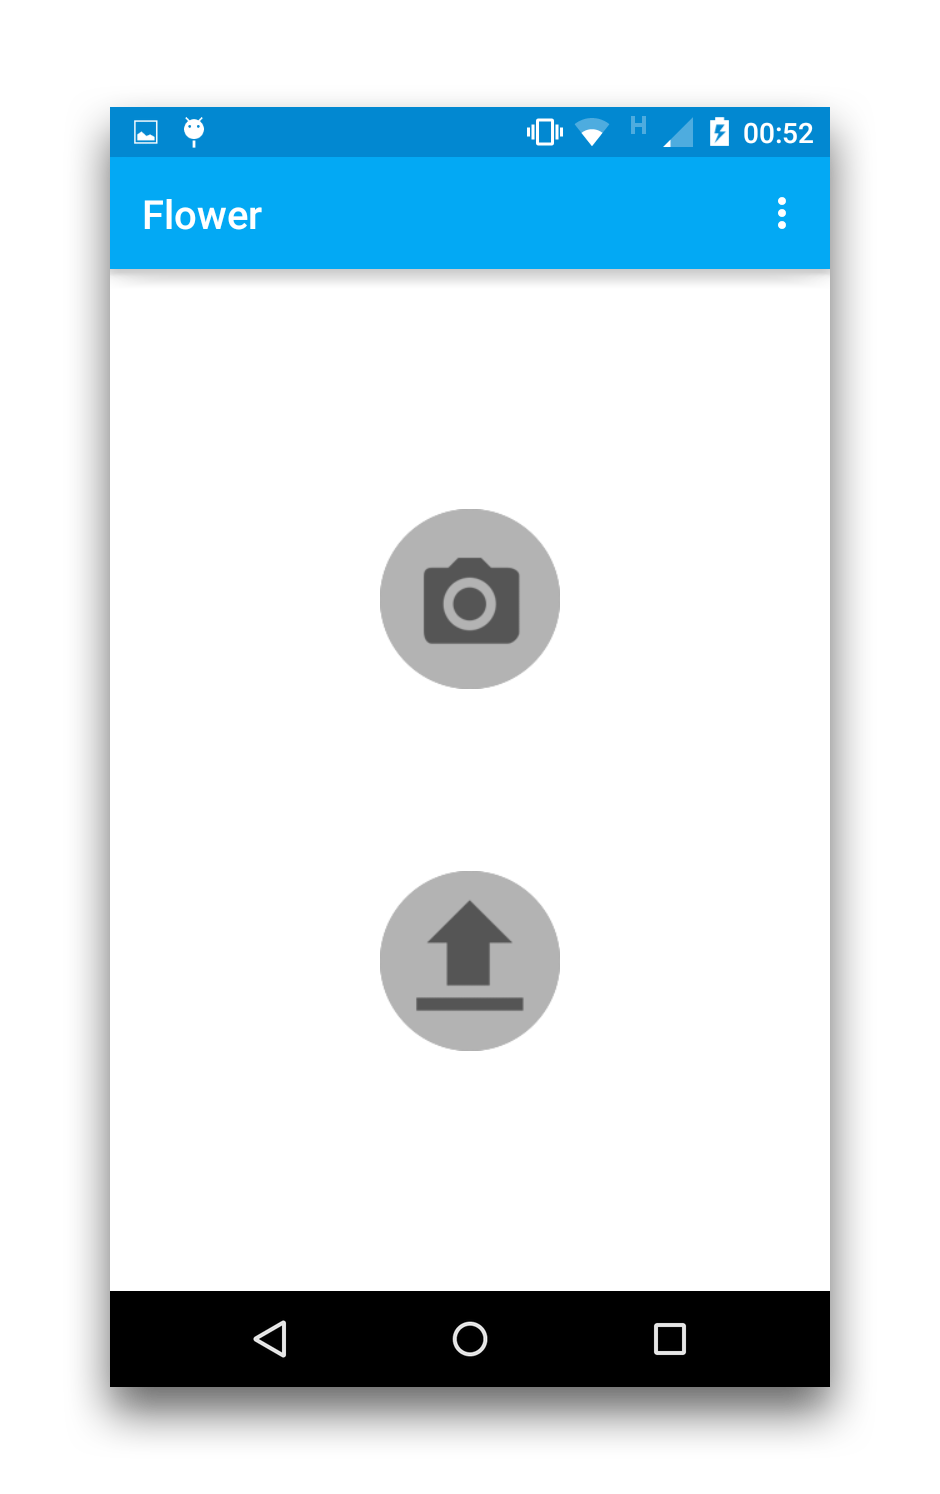
\includegraphics[totalheight=6cm]{img/47.png}
	(a)
\end{minipage}
\begin{minipage}[b]{0.2\linewidth}
	\centering
	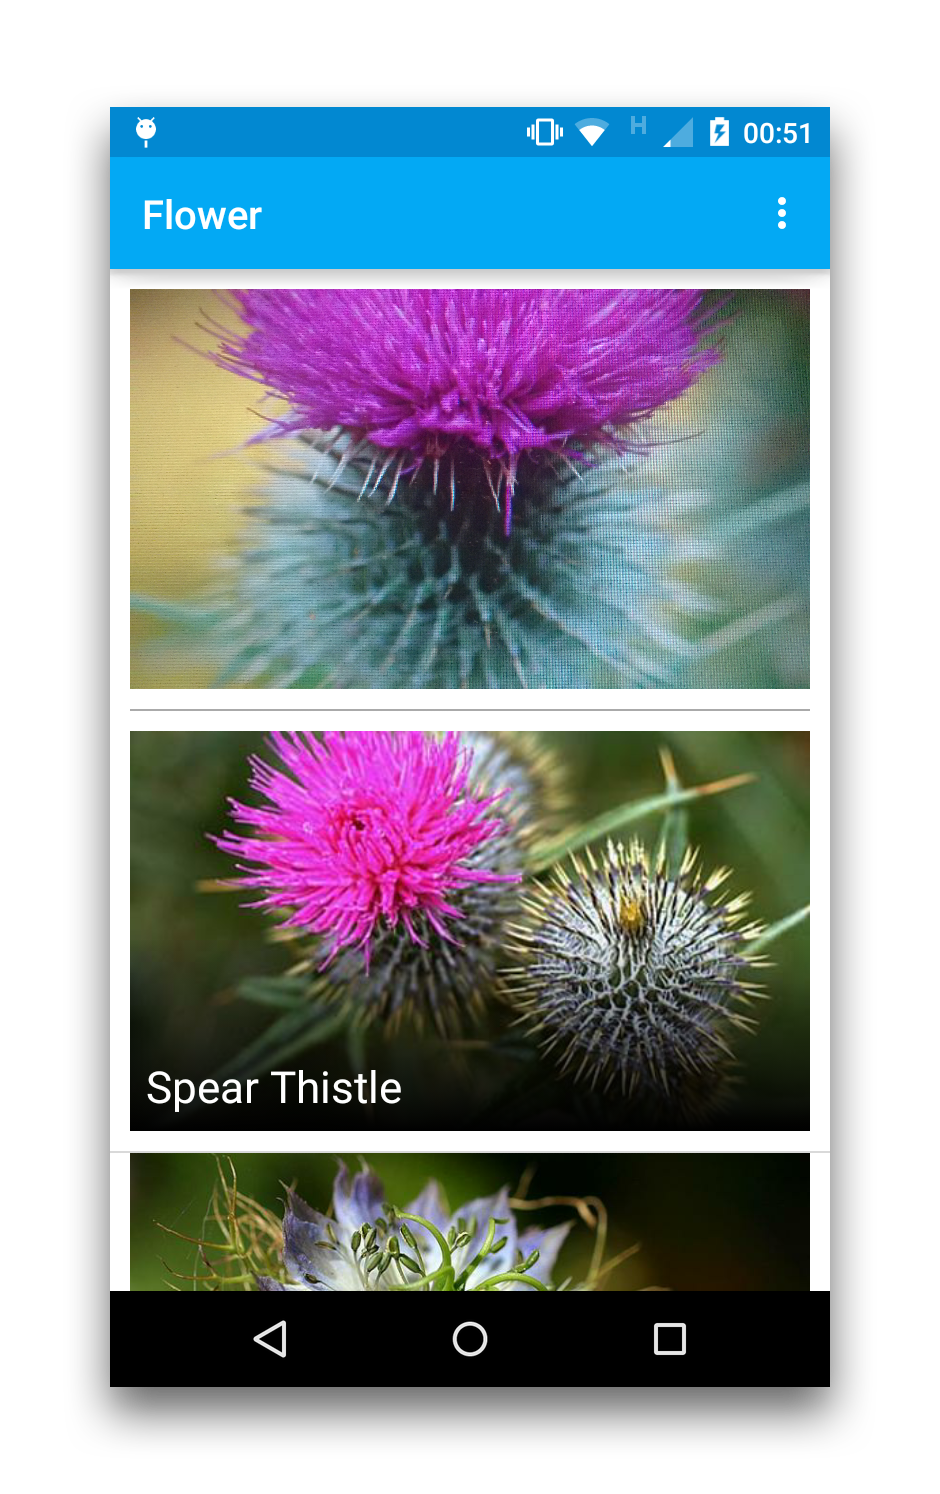
\includegraphics[totalheight=6cm]{img/48.png}
	(b)
\end{minipage}
\begin{minipage}[b]{0.2\linewidth}
	\centering
	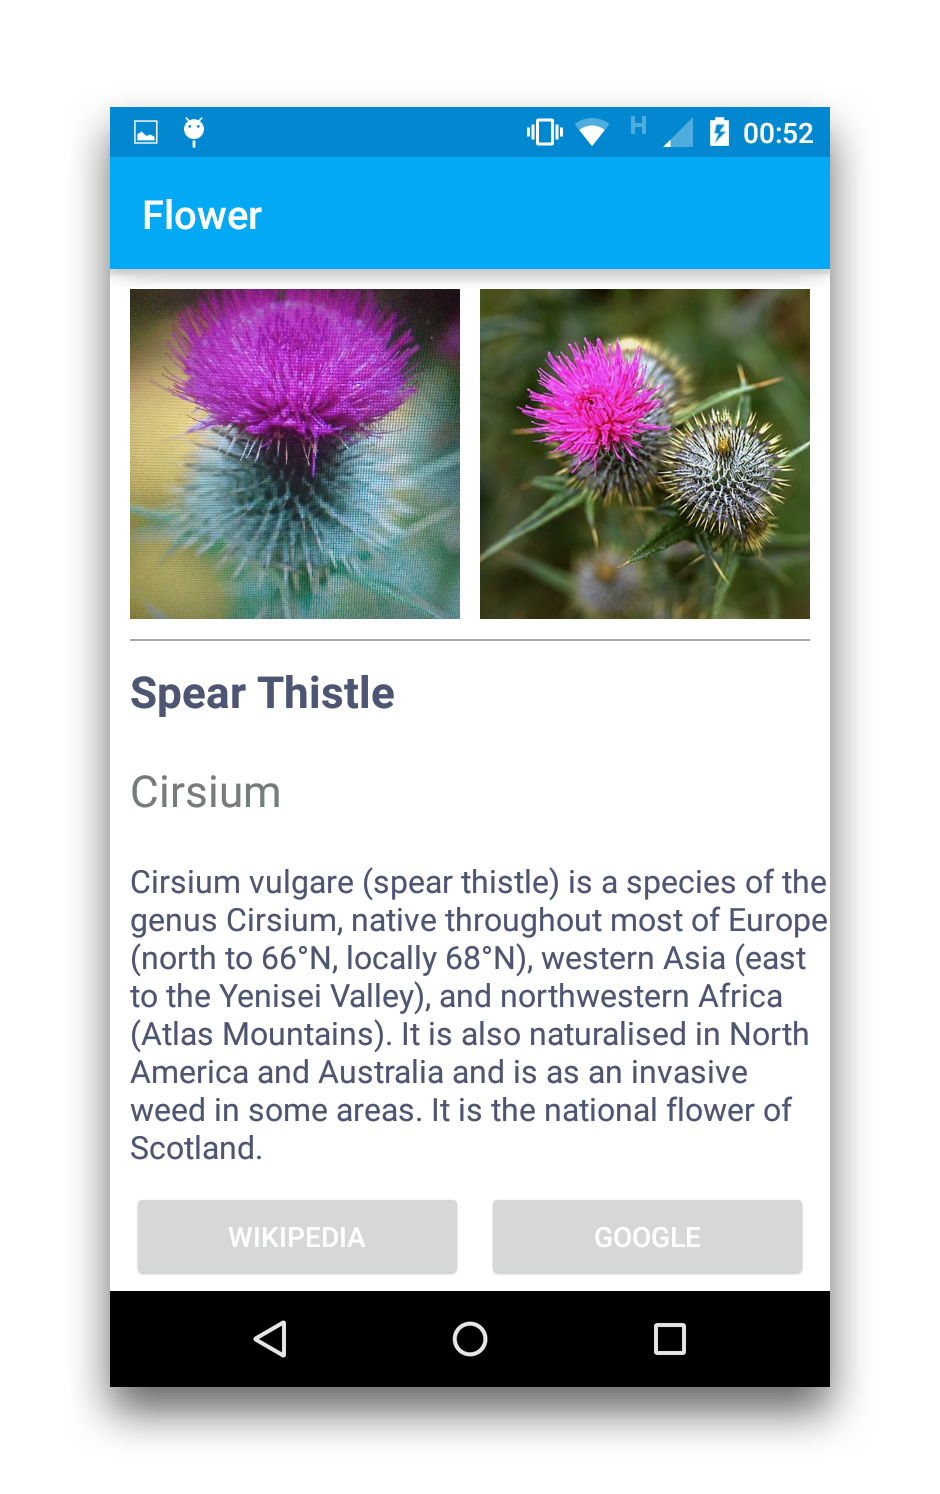
\includegraphics[totalheight=6cm]{img/49.png}
	(c)
\end{minipage}
\caption{Screenshots of the screens seen by user. (a): The user chooses whether to take or upload a photo. (b): The photo is automatically uploaded, classified and the results of the classification are displayed. (c): If one of the images in (b) is clicked, a detailed view of that flower is shown. The flower's common name, genus, a snippet from information from Wikipedia and buttons linking to the flower's Wikipedia and Google Search pages are displayed.}
\label{img:47}
\end{figure}


For the user, the application is simple. A photo is taken, it is automatically uploaded and classified, and the six top classification predictions are presented to the user, who makes the final decision. 

The classification itself is an automated process. After the photo is uploaded to a server, it is passed to a convolutional neural network which outputs a vector describing the features, such as shape and colour, of the photo. This feature vector is compared to a previously trained support vector machine model of 102 common flower species. A ranked list of the six most similar flowers from the 102 is returned to the application and presented in a clear and intuitive manner. 

This application implements fine-grained classification, that is classification between categories which are visually and semantically similar. Although flowers are the chosen classification subject of this project, the same techniques could successfully be applied to other fine-grained classification tasks. 

\section{Road map}

This report consists of six chapters. In Chapter 2, the literature review examines previous work which is relevant, including work done by Oxford University on the flower classification problem and applications of a similar nature. This chapter also reviews the convolutional neural network algorithm which is used to extract features from the flower image.

Chapter 3 considers the flower classification. The two-step system of convolutional neural network based feature extraction and support vector machine classification is laid out. The experiments carried out to fine tune the classification system and the results obtained are also covered. 

%TODO fix this
In Chapter 4, the client (application) and server architecture are examined. The process by which the user takes and uploads the photo, how the classification process is implemented and the communication between client and server are detailed. 

Chapter 5 looks at application design and looks at the user interface and user experience. While chapter four covered the mechanics of how the application works, this chapter considers its look and feel.

Finally, Chapter 6 presents a summary of this project and discusses further work which can be carried out on this topic.




%-------------------------------
% Literature Review
%-------------------------------
\chapter{Literature review}

% (3-5 pages long. Gives reader knowledge of what people have done before on this topic.) 

This chapter considers the previous work relevant to the project. It gives a description of the data used, looks at the work done at Oxford University on this particular problem, the history of the algorithms used, and other applications which solve similar problems. 


\section{Description of data}

\begin{figure}[hbt]
	\centering
  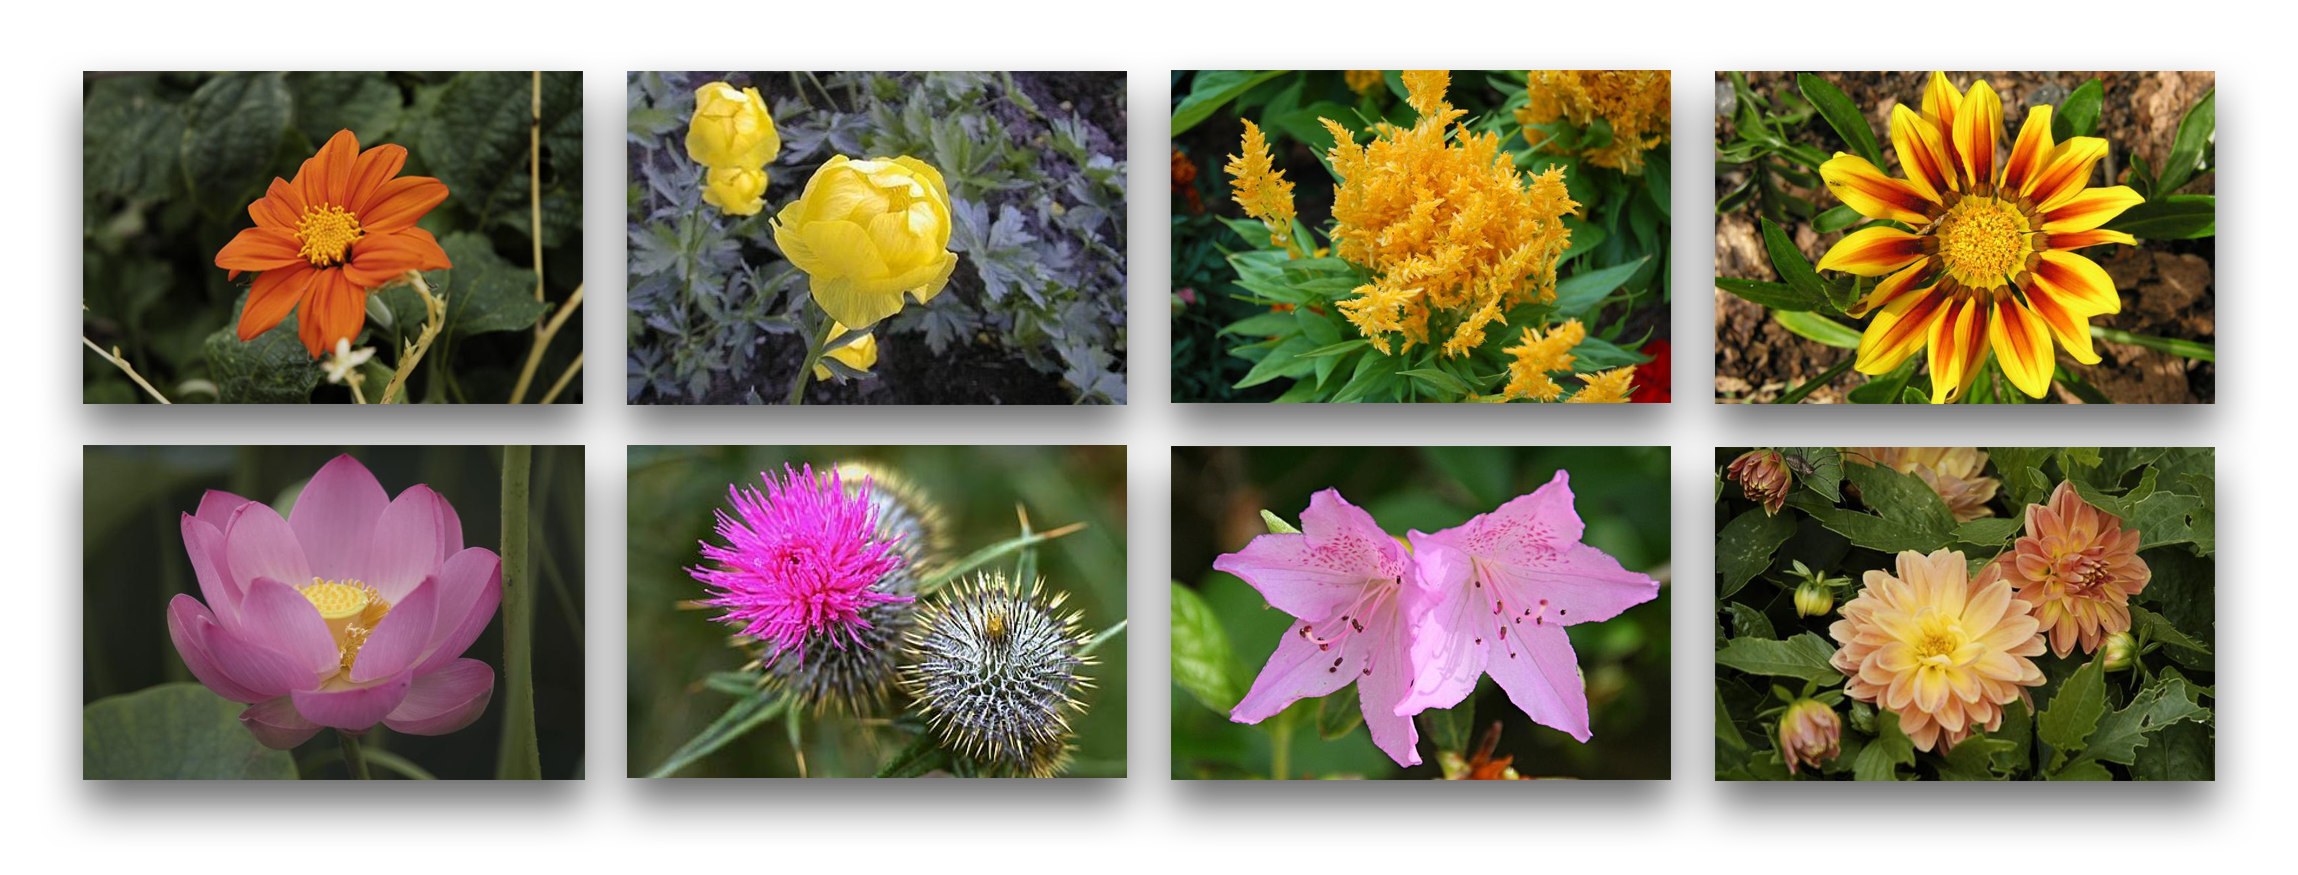
\includegraphics[totalheight=6cm]{img/26.png}
  \caption{Example images from the 17 and 102 flower datasets}
  \label{img:26}
\end{figure}

This project makes use of the Oxford 17 category flower dataset\footnote{http://www.robots.ox.ac.uk/~vgg/data/flowers/17} and the Oxford 102 category flower dataset\footnote{http://www.robots.ox.ac.uk/~vgg/data/flowers/102}. Example images from the datasets are shown in Figure~\ref{img:26}. The 17 flower dataset is split into 17 flower species, each containing 80 images. The 102 flower dataset is split into 102 flower species, each  containing between 40 and 258 images.

The flower species in both sets are common to the United Kingdom, and the photos exhibit variations in pose and light levels. Both include species which exhibit great variation within the species and species which look similar to others in the dataset, shown in Figure~\ref{img:33}.

The datasets are split into training, validation and test sets, and the categories themselves are numbered 1 to 17 and 1 to 102 respectively. A data file which relates these these category numbers to an appropriate genus, species and common name is used to present meaningful information to the user. 


\section{Flower Classification}

This project builds on work done by the Oxford University Visual Geometry Group on the flower classification problem. Nilsback et al.~\cite{Nilsback08} considered how combinations of features (local shape/texture, shape of the boundary, overall spatial distribution of petals, and colour) affect classification accuracy. After feature extraction has taken place, a support vector machine (SVM) classifier is used. When tested against the Oxford 102 flower dataset, a classification accuracy of 72.8\% was obtained.

 Chai~\cite{LitRev:Chai} uses a flower classification method which involves segmenting each flower image into foreground (the flower itself) and background, before using Fisher vectors to extract flower features. An example of the image segmentation is shown in Figure~\ref{img:34}. An SVM classifier was also used to achieve classification accuracy of 81.4\% when tested on the Oxford 102 flower dataset.  
 
\begin{figure}[hbt]
	\centering
  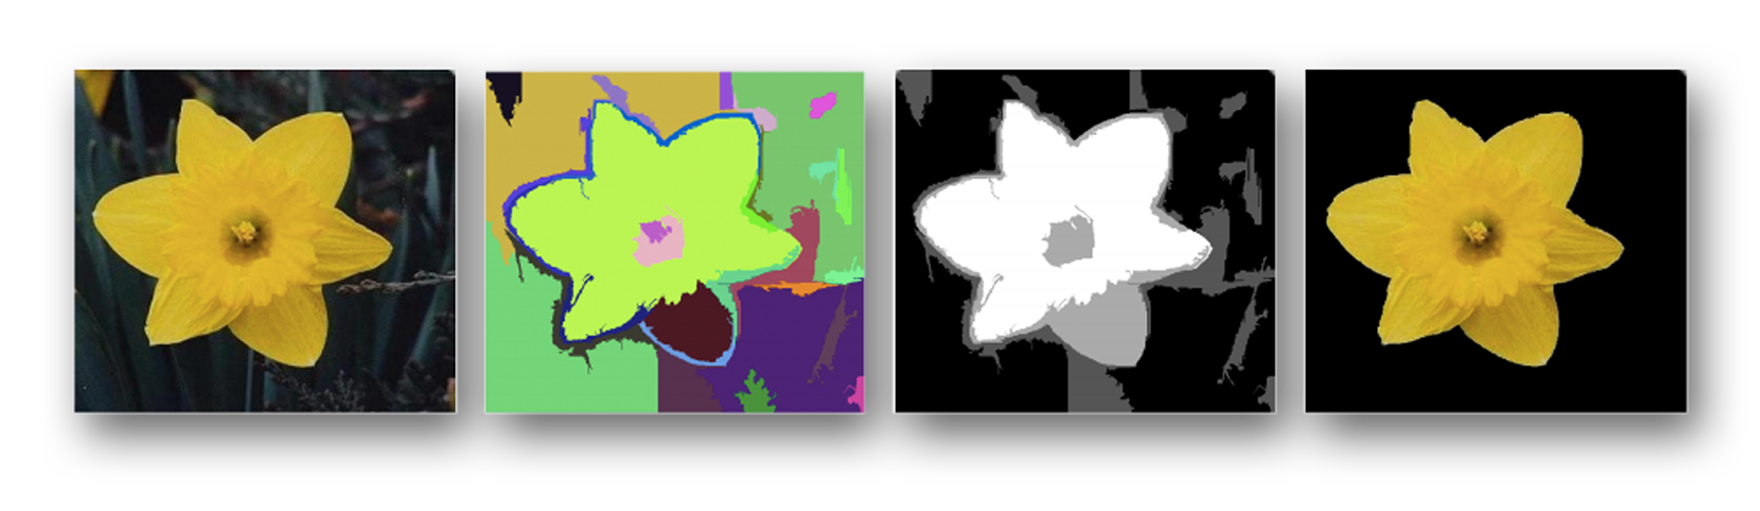
\includegraphics[totalheight=4cm]{img/34.png}
  \caption{Image segmentation from ~\cite{LitRev:Chai}}
  \label{img:34}
\end{figure}
 
\section{Convolutional Neural Networks}

%\textbf{Todo: explain layers and how it’s convolutional}

This project takes a different approach to Chai and Nilsback, making use of a convolutional neural network (CNN) for feature extraction. CNNs are a type of biologically-inspired neural network, based on the multilayer perceptron~\cite{LitRev:DeepLearning}.


A CNN takes an input vector and transforms it to an output vector by passing it though several hidden layers each made up of a set of neurons. It can be thought of as a function $f$ which transforms an input $\vect{x}$ into an output $\vect{y}$. The function $f$ is in fact made up of a sequence of simpler functions $f_1, f_2, ..., f_N$~\cite{arXiv:1412.4564}. Each function $f(\vect{x}, \vect{w})$ has a set of parameters $\vect{w}$ which are determined during training. 

\begin{figure}[hbt]
	\centering
  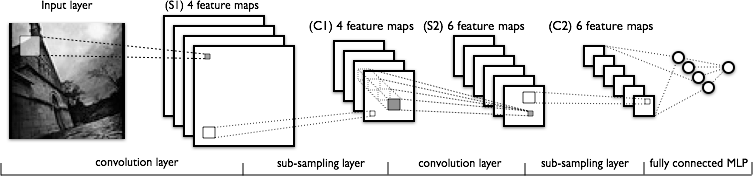
\includegraphics[totalheight=3cm]{img/52.png}
  \caption{Diagram showing the layers in a convolutional neural network}%\footnote{http://deeplearning.net/tutorial/lenet.html} }
  \label{img:52}
\end{figure}
%CNNs, where they came from, who invented them, imagenet challenge (\url{http://www.image-net.org/}), image depicting CNN architecture. 


\section{Automatic visual classification applications}

Automatic flower classification applications do not exist at the time of writing, but there are several applications which use computer vision techniques to classify subjects such as tree species and dog breeds.

The iPhone application Leafsnap~\cite{leafsnap_eccv2012} uses computer vision to automatically identify 	tree species using photographs of leaves. The leaf shape is used as the principle feature, and shape is obtained by using colour-based segmentation to remove the background from the image of the leaf before taking multiscale curvature measures. For optimal use, the leaf must be placed on a white sheet of paper before the image is taken. The flowers are classified from this data by using nearest-neighbour classification. The application currently classifies the 185 tree species in the Northeastern United States. 

\begin{figure}[hbt]
	\centering
  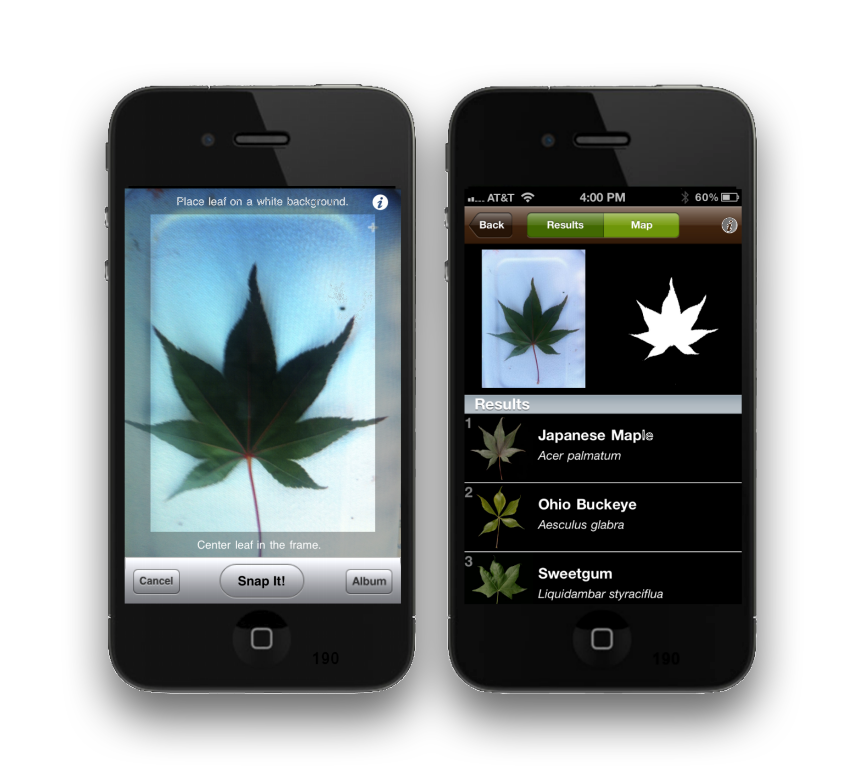
\includegraphics[totalheight=8cm]{img/35.png}
  \caption{Screenshots of the image capture and results screens from the Leafsnap application~\cite{leafsnap_eccv2012}}
  \label{img:35}
\end{figure}

The application makes use of a client-server architecture, where the classification takes place on Leafsnap's servers. The classification time for a single photo is 5.4 seconds, not including upload time. It also implements a 'field guide' containing images and descriptions of the trees it classifies.

The group which produced Leafsnap, Columbia University, The University of Maryland and The Smithsonian Institution have released another automatic image classification application called Dogsnap, which classifies dog breeds.

Dogsnap uses greyscale SIFT descriptors and a colour histogram to extract features from the photograph and uses a one-vs-the-rest SVM for classification~\cite{conf/eccv/LiuKJB12}. Dogsnap uses relative eye and nose position as the principle features as they are rigid in relation to one another. 


\section{Flower classification applications}

Several basic flower classification application have been created which do not use image-based automatic classification. These fall into two categories; digital field guides and human powered classification.


The former provide an extensive database of plant species and allow the user to manually narrow down their search based on distinguishing plant features\footnote{https://play.google.com/store/apps/details?id=com.luontoportti}\footnote{https://itunes.apple.com/us/app/ipflanzen/id416983587}, or by user location\footnote{https://play.google.com/store/apps/details?id=org.pottssoftware.agps21}. These are usually free and represent a significant improvement on paper field guides; they are more portable, easier to search and as most people carry phones they are usually to hand when needed. 

The latter allows the user to take a photograph of the flower in question and upload it to a platform where it is manually classified by a person\footnote{https://play.google.com/store/apps/details?id=org.plantnet}\footnote{https://play.google.com/store/apps/details?id=cz.thran.flowerchecker}. Applications of this nature differ in who is used to classify the flower. Some crowdsource information from the users of the application. This is usually free but the results are potentially unreliable, the application requires a large user base to work and classification time can take up to days. Others use a team of professionals which is more reliable and potentially faster but requires payment.












%-------------------------------
% Classification
%-------------------------------
\chapter{Classification}
\label{sec:classification}


%TODO say that this chapter includes testing etc
%TODO say briefly why classification result is important - affects quality of the whole application
This chapter describes the classification pipeline and the experiments done on it. The classification pipeline takes an image as its input and outputs a classification result. The process is summarised in Figure~\ref{img:08}. This description is mostly theoretical, details of its implementation are covered in Chapter~\ref{sec:client_server}. High classification accuracy is crucial for the quality of this application. 

\begin{figure}[hbt]
	\centering
  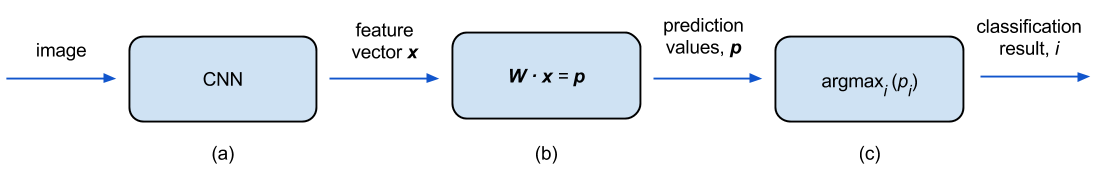
\includegraphics[totalheight=3cm]{img/08.png}
  \caption{(a): Convolutional neural network inspired feature extraction. An image is supplied to the convolutional neural network which generates its feature vector $\vect{x}$, which describes the content of the photograph. (b): Support vector machine image classification. The vector is compared to the previously found weight vectors $\vect{W}$, producing a vector of prediction values, $\vect{p}$. (c) The index $i$ of the maximum value in $\vect{p}$ is found, which gives the classification result $i$.}
  \label{img:08}
\end{figure}


\section{Convolutional neural network (CNN) based feature extraction}

The pipeline makes use of the first six layers of the fast convolutional neural network CNN-F introduced in Chatfield et al.~\cite{Chatfield14}. This algorithm takes a photo of size 244x244 pixels as its input and produces a vector $\vect{x}$ which describes the features of the photo. The feature vector is 4096 dimensional and is $l_2$ normalised before being passed to the support vector machine (SVM), as SVMs work best with $l_2$ normalised vectors.

The CNN is trained on the ImageNet Large Scale Visual Recognition Challenge 2012 (ILSVRC2012) dataset~\cite{CNN:Imagenet}. Details of the training can be found in Chatfield et al.~\cite{Chatfield14}. The feature extraction process itself is treated as a black box in this project. 

 


\section{Support vector machine (SVM) image classification}

\subsection{How SVMs are used in the classification pipeline}

The classification pipeline uses the open source support vector machine (SVM) library LibLinear~\cite{REF08a} for quick, large scale classification. One-vs-the-rest classification is used. $N$ SVM models are trained for $N$ flower categories, producing $N$ weight vectors, $\vect{w_{1}}, \vect{w_{2}}, ..., \vect{w_{N}}$. These weight vectors are stacked into a weight matrix $\vect{W}$: 
$$
\vect{W} = 
\begin{pmatrix}
\vect{w_{1}'}\\  
\vect{w_{2}'}\\ 
\vdots \\ 
\vect{w_{N}'}
\end{pmatrix}
$$



During classification, the scalar product of the unseen flower's feature vector, $\vect{x}$ and each of the weight vectors is calculated, to produce a vector of prediction values, $p_{1}, p_{2} ... p_{n}$:
$$
\vect{W} \cdot \vect{x} =
\begin{pmatrix}
p_{1}\\  
p_{2}\\ 
\vdots \\ 
p_{N}
\end{pmatrix}
$$

The value of $p_{i}$ indicates how similar the unseen flower's features were to those of category $i$. The higher the product, the more similar they are. A ranked list of categorisation possibilities is calculated by ordering the prediction values by size. 


\subsection{Training and testing SVMs}

Before use, the SVM models $\vect{w_{1}}, \vect{w_{2}}, ..., \vect{w_{N}}$ which make up $\vect{W}$ must be trained. They are trained using a set of images which are known to be of certain categories. The models are then tested, using a set of images also known to be of certain categories, to check they are sufficiently accurate.


\subsubsection{Training} 

The SVM models are trained using LibLinear's training function. To train a model to recognise a flower category $i$, all photos in the training and validation sets are passed to the training function, with the photos of category $i$ labeled as in the category, and all other flowers labeled as not in the category. The flowers are labeled as in or not in the category by passing a 1 or -1 respectively to the training function, alongside that flower's feature vector.

The training function produces a weight vector of dimension 4096, which describes the characteristics of the flowers in that category. 

The $C$ parameter of the SVM must be adjusted during training. The $C$ parameter allows for a solution with a larger margin, in return for the violation of some constraints. This can improve classification accuracy. To find the optimal $C$ parameter, SVM models are trained using the training set images  before being tested against the validation set images. The change in classification accuracy is recorded as the $C$ parameter is changed. Figure~\ref{img:27} shows how the accuracy changes as the $C$ parameter is changed. Based on this graph, a $C$ parameter of $10^3$ was chosen for the the 17 flower dataset with no test or training set augmentation (explained in Section~\ref{sec:augmentation}). 

\begin{figure}[hbt]
	\centering
  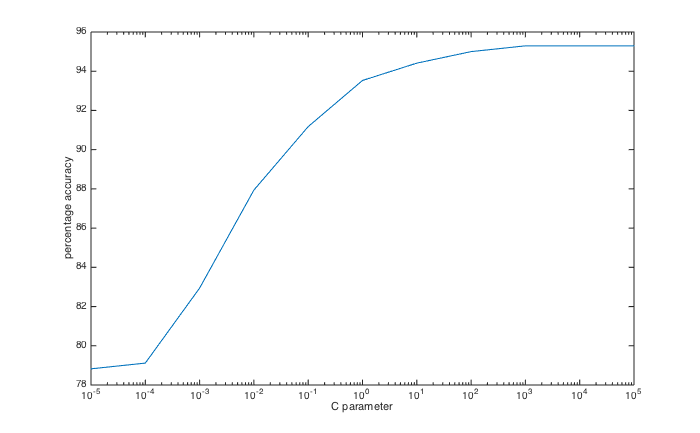
\includegraphics[totalheight=10cm]{img/27.png}
  \caption{Graph showing how accuracy changes as the $C$ parameter is changed for the 17 flower dataset with no test or training set augmentation. Image augmentation is explained in Section~\ref{sec:augmentation} }
  \label{img:27}
\end{figure}

\subsubsection{Testing}

Testing allows the quality of each SVM model to be checked. Testing uses the test subset of the flower datasets. Each flower in the test set is run against each of the SVM models generated during training. The dot product of the  flower's feature vector and each of the model's weight vectors is found. The greater the result of the dot product, the greater the correlation between the tested flower and that category. Thus the category which produces the greatest dot product result is predicted to be the category of the flower.

By comparing the actual categories of the flowers in the test set to the predicted categories, an overall percentage accuracy can be calculated.


\section{Experiments}
%aim to make this section 7 pages

This section describes the metrics used, experiments run and results obtained whilst testing the quality of the classification pipeline. 

\subsubsection{Accuracy}

To calculate an overall accuracy, the accuracy of each model must first be calculated. The overall accuracy is then defined as the mean of the model accuracies:

$$
\text{Overall accuracy}  = \frac{\text{Sum of model accuracies}}{\text{Number of flower categories}}
$$

Model accuracy is defined as:
$$
\text{Model accuracy} = \frac{\text{Number of correctly classified flowers}}{\text{Number of flowers classified}}
$$

\subsubsection{Rank accuracy}

Rank accuracy measures the accuracy when considering the top $K$ predicted categories, as demonstrated in Figure~\ref{img:50}. 
$$
\text{Rank accuracy}  = \frac{\text{Sum of model accuracies when considering the top } K \text{results}}{\text{Number of flower categories}}
$$

\begin{figure}[hbt]
	\centering
  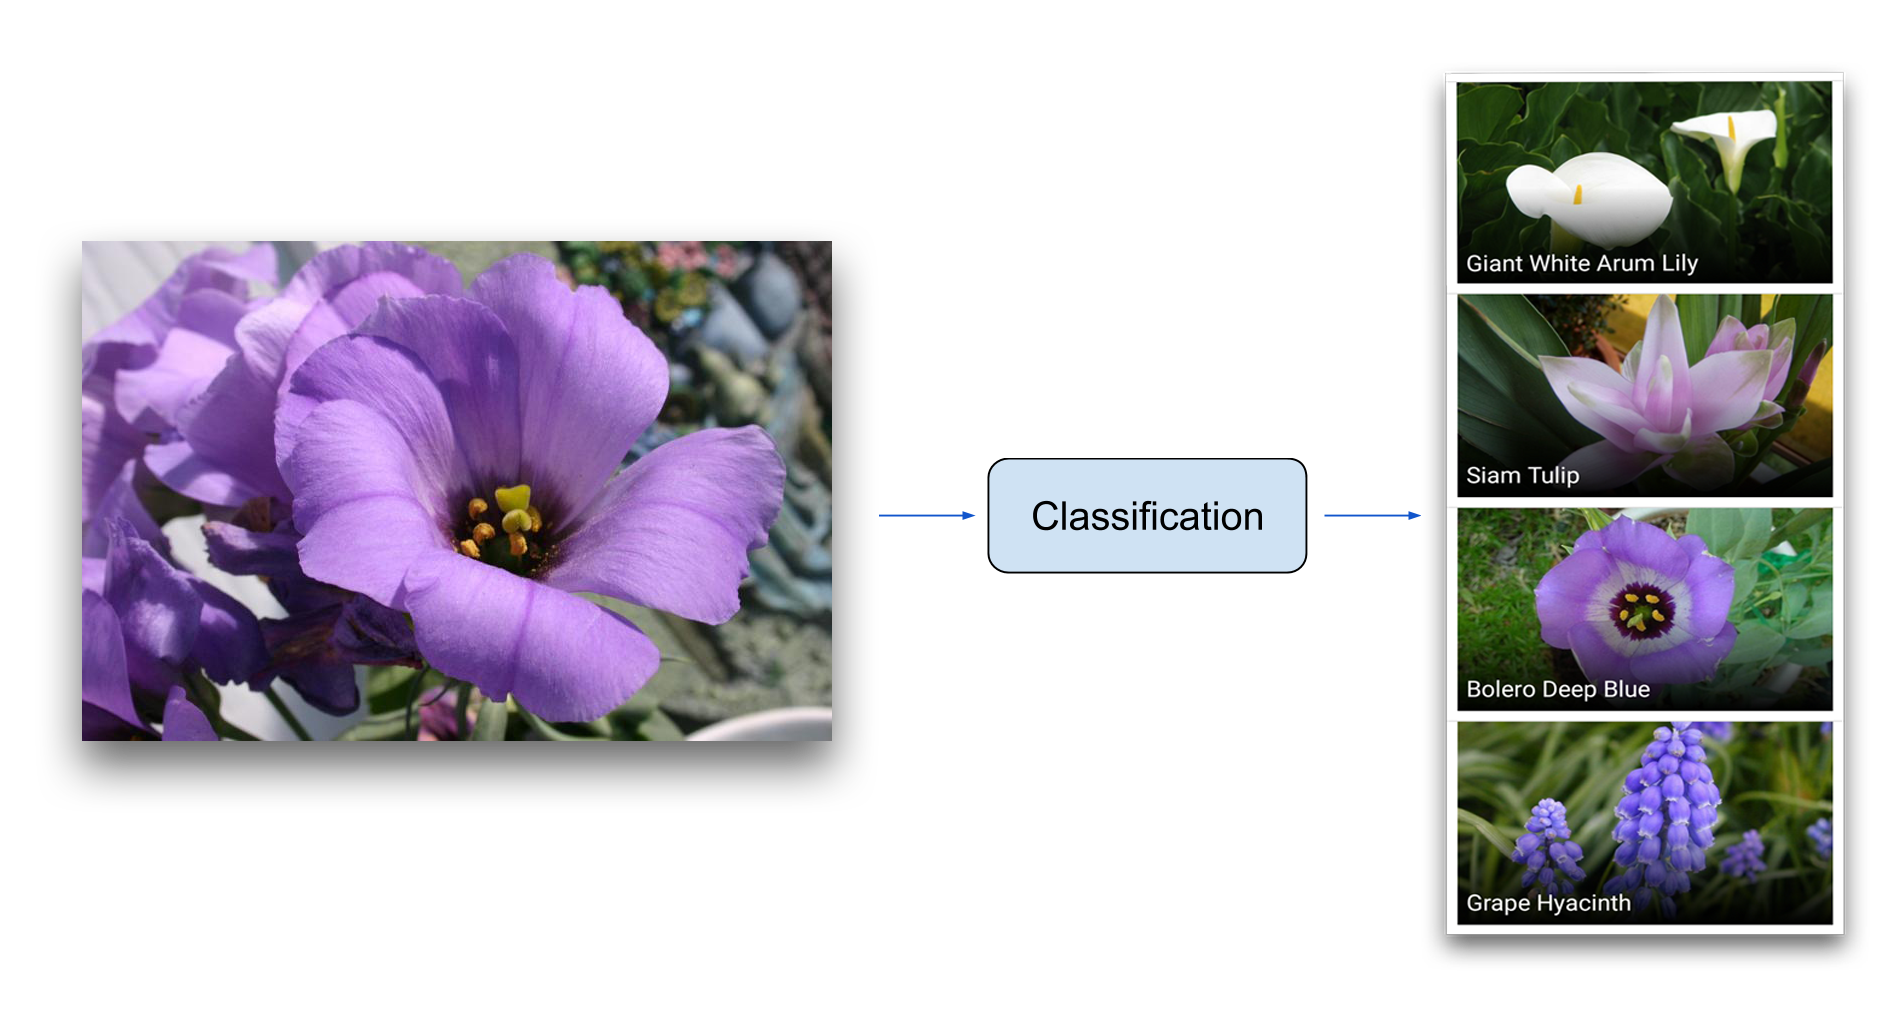
\includegraphics[totalheight=8.5cm]{img/50.png}
  \caption{Diagram demonstrating rank accuracy. Left: A bolero deep blue flower is being classified. Right: The ranked classification predictions. The accuracy is 0\% when considering the first rank ($K = 1$), 0\% when considering the first two ranks ($K = 2$), and 100\% when considering $K = 3$ and $K = 4$.}
  \label{img:50}
\end{figure}



\subsection{Results}

\begin{table}[h]
\centering 
\renewcommand{\arraystretch}{1.3}
\begin{tabular}{c|cc}
  & {\bf 17 flower dataset} & {\bf 102 flower dataset} \\
  \hline
  Baseline & 89.3 $\pm$ 0.96\% & 85.7 $\pm$ 0.92\% \\
  Mirroring & 89.1 $\pm$ 0.93\% & 85.2 $\pm$ 0.30\% \\
  Sampling & 89.1 $\pm$ 1.06\% & 84.3 $\pm$ 0.13\% \\
  Mirroring and Sampling & 89.7 $\pm$ 1.21 \% & 84.7 $\pm$ 0.43\% 
\end{tabular}
\renewcommand{\arraystretch}{1}
\caption{Mean classification accuracy and standard deviation for the Oxford 17 and 102 flower datasets using training set augmentation (Section~\ref{sec:train_augmentation}), and not using test set augmentation (Section~\ref{sec:test_augmentation})}
\label{table:accuracy}
\end{table}

\begin{table}[h]
\centering 
\renewcommand{\arraystretch}{1.3}
\begin{tabular}{c|cc}
  {\bf Number of}\\ {\bf ranks considered} & {\bf 17 flower dataset} & {\bf 102 flower dataset} \\
  \hline
  1 & 89.7\% & 84.7\% \\
  4 & 98.6\% & 94.7\% \\
  6 & 99.1\% & 96.2\% \\
  8 & 99.6\% & 97.1\% \\
  10 & 99.8\% & 97.6\% 
\end{tabular}
\renewcommand{\arraystretch}{1}
\caption{Classification accuracies obtained when considering different numbers of ranks for the 17 and 102 flower datasets, using training set augmentation}
\label{table:rank}
\end{table}


Table~\ref{table:accuracy} shows the percentage accuracy for the 17 and 102 flower datasets when using training set augmentation. Table~\ref{table:rank} shows the percentage rank accuracy for the 17 and 102 flower datasets when using training set augmentation. To improve the reliability of the accuracy results, each experiment is run five times, using a randomly generated training set of 20 images from each category. The test set is made up of all the remaining images. 


\subsection{Analysis of results}

\subsubsection{Accuracy}

The highest accuracies obtained for the 17 flower and 102 flower datasets are 89.7\% and 85.7\% respectively. A lower accuracy for the 102 flower dataset is to be expected as there are more classification possibilities. The accuracy for the 102 flower set is 4 percentage points higher than those obtained in Chai~\cite{LitRev:Chai} and 13 percentage points higher than those obtained in Nilsback et Al.~\cite{Nilsback08}. The standard deviations of the results are low, indicating that the accuracy figures are reliable. These accuracies are obtained using models trained on a subset of the total images available. The final models used for the application are trained on all the images, and should have higher accuracy rates.

Mirroring and sampling increase the size of the training set and can improve classification accuracy, as seen in~\cite{Chatfield14}. However, this was not seen in these results.

\subsubsection{Rank accuracy}


The rank accuracy graph shows that classification accuracy quickly increases as more ranks are considered (Table~\ref{table:rank}). While the accuracy is a useful metric for understanding the quality of the models, rank accuracy gives a better insight into the accuracy experienced by the user as they are presented with the top $K$ classification results by the application. The value of $K$ is a compromise between accuracy and complexity; the more results presented to the user, the greater the likelihood of the correct result being in the list but at some point the extra information becomes confusing. 

A value of $K = 6$ was settled on as it gives a high accuracy of 96.2\% for the 102 flower dataset and six is a very manageable number of options for a user to be presented with. Figure~\ref{img:30} shows that considering further ranks yields a greatly diminished increase in accuracy. Offering the user a smaller number of options has the added benefit of reducing the amount of data needed by the application per classification, speeding up the classification.


\begin{figure}
\centering
\begin{minipage}{.45\textwidth}
  \centering
  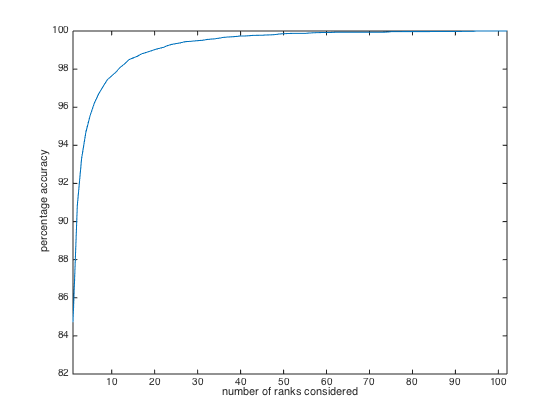
\includegraphics[width=1\linewidth]{img/29.png}
  \captionof{figure}{Rank accuracy for 102 flower dataset, using training set augmentation}
  \label{img:29}
\end{minipage}%
\begin{minipage}{.1\textwidth}
~ % Used to force a gap between the images
\end{minipage}%
\begin{minipage}{.45\textwidth}
  \centering
  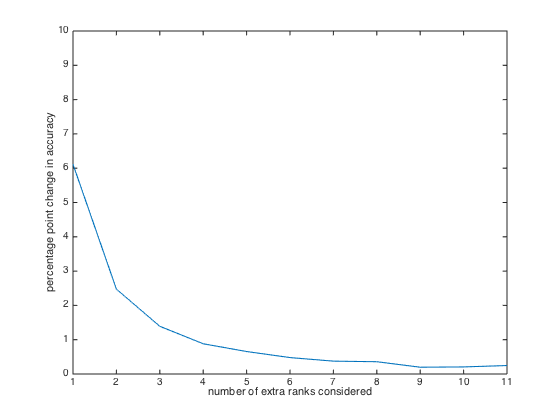
\includegraphics[width=1\linewidth]{img/30.png}
  \captionof{figure}{Percentage point increase in accuracy when considering more ranks }
  \label{img:30}
\end{minipage}
\end{figure}



\subsubsection{Test set augmentation}

\begin{table}[h]
\centering 
\renewcommand{\arraystretch}{1.3}
\begin{tabular}{c|cc}
  & {\bf 17 flower dataset} & {\bf 102 flower dataset} \\
  \hline
  Baseline & 89.1 $\pm$ 0.12\% & 85.7 $\pm$ 0.92\% \\
  Mirroring & 88.9 $\pm$ 0.12\% & 85.7 $\pm$ 0.10\% \\
  Sampling & 90.1 $\pm$ 1.23\% & 86.7 $\pm$ 0.40\% \\
  Mirroring and Sampling & 89.7 $\pm$ 0.66 \% & 85.3 $\pm$ 0.44\% 
\end{tabular}
\renewcommand{\arraystretch}{1}
\caption{Mean classification accuracy and standard deviation for the Oxford 17 and 102 flower datasets using test set augmentation (Section~\ref{sec:test_augmentation})	, and not using training set augmentation (Section~\ref{sec:train_augmentation})}
\label{table:test_augmentation}
\end{table}


Test set augmentation, explained in Section~\ref{sec:test_augmentation}, gave the results shown in Table~\ref{table:test_augmentation}. Although a slight improvement is seen, test augmentation requires the CNN based feature extraction to be run multiple times. As the feature extraction is the most time costly part of classification, test image augmentation increases classification time by up to 3.6 times, as shown in Table~\ref{table:classification_time}. For this reason, test image augmentation is not implemented in the classification pipeline.



\begin{table}[h]
\centering 
\renewcommand{\arraystretch}{1.3}
\begin{tabular}{c|cc}
  & {\bf Classification time / seconds} \\
  \hline
  Baseline & 0.97 \\
  Mirroring &  1.03 \\
  Sampling & 2.98  \\
  Mirroring and Sampling & 3.64
\end{tabular}
\renewcommand{\arraystretch}{1}
\caption{ Classification time when using test image augmentation. These results were obtained by timing the Matlab classification script from within Matlab. Actual classification times will be longer due to additional server computation, image upload and classification information download time. }
\label{table:classification_time}
\end{table}

\subsubsection{Confusion matrices}

Confusion matrices give a more detailed view of the classification. It presents the classification results as a series of rows. Each row represents all of the images in the test dataset for that category. The numbers in the columns represent the proportion of those images which were classified as that category. For example, for the 17 flower dataset confusion matrix, shown in Figure~\ref{img:31}, 45\% of the images of category 1 in the training set were correctly classified. 3\% were incorrectly classified as category 6, 15\% as 9 and 38\% for 14.

The 17 flower confusion matrix (Figure~\ref{img:31}) shows that most of the individual classification models perform well, with all but four showing accuracies greater than 70\%. However, it can be seen that categories 1, 8 and 15 perform much worse than expected, with accuracies between 40\% and 45\%. All three of these categories have significant numbers of images (between 38\% and 53\%) misclassified to category 14, and some images from category 1 are misclassified to category 8.

\begin{figure}[hbt]
	\centering
  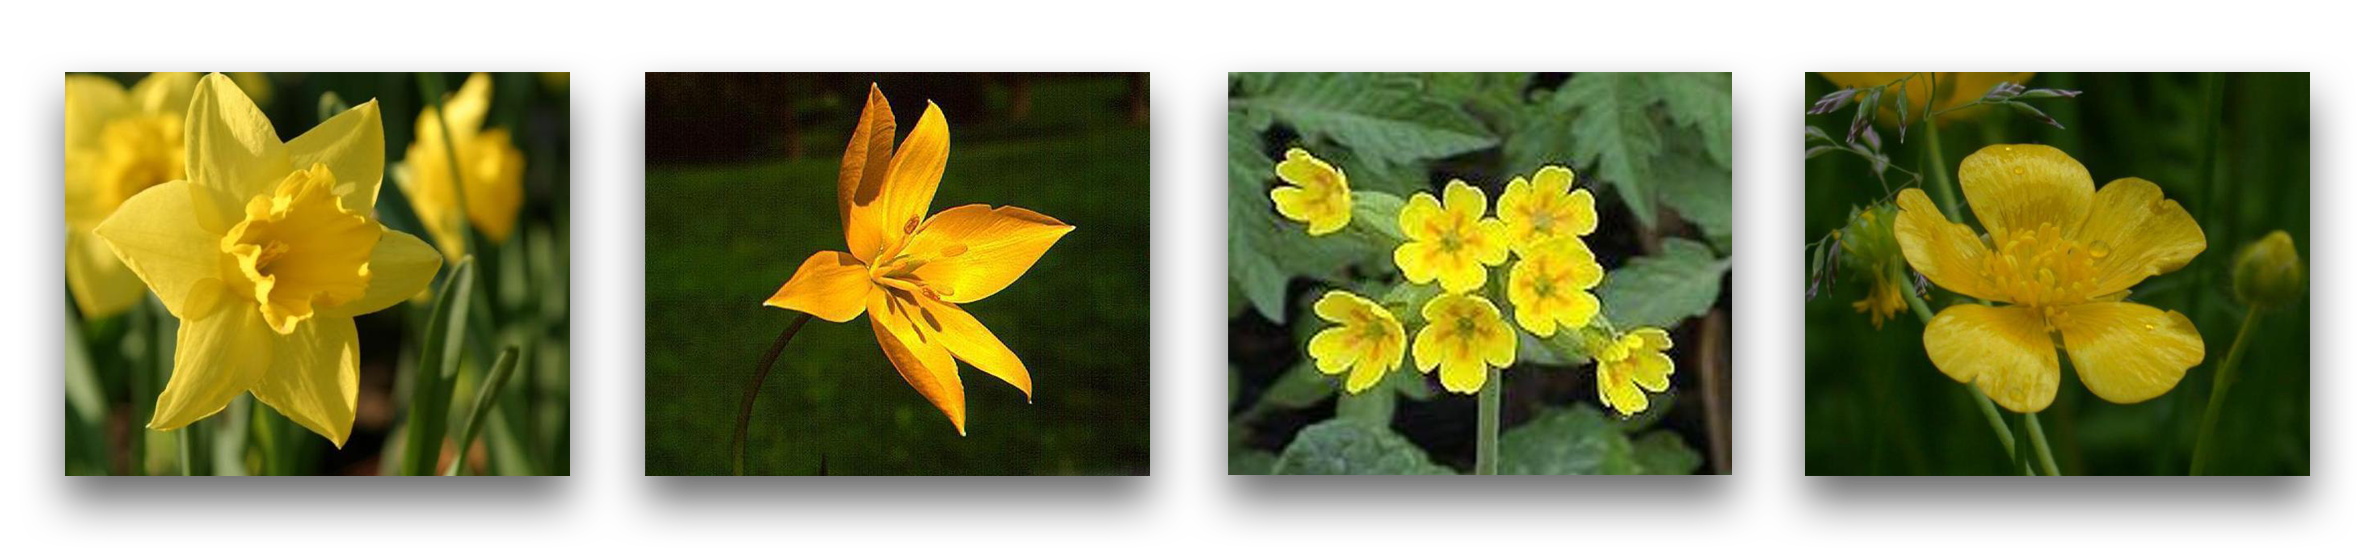
\includegraphics[totalheight=4cm]{img/36.png}
  \caption{Example images from categories 1, 8, 14 and 15. The flowers are similar and there is misclassification between classes.}
  \label{img:36}
\end{figure}

One can see that by looking at images of the flowers in question, shown in Figure~\ref{img:36}, that they all look similar, with yellow petaled flowers on mostly green backgrounds. This similarity explains the confusion, which is mostly corrected for when considering rank accuracy. 

Category 6, the sword lily shows large colour variation within the species, shown in Figure~\ref{img:37}. However, the high accuracy of 85\% indicates that the these problems are effectively handled by the classification pipeline.

\begin{figure}[hbt]
	\centering
  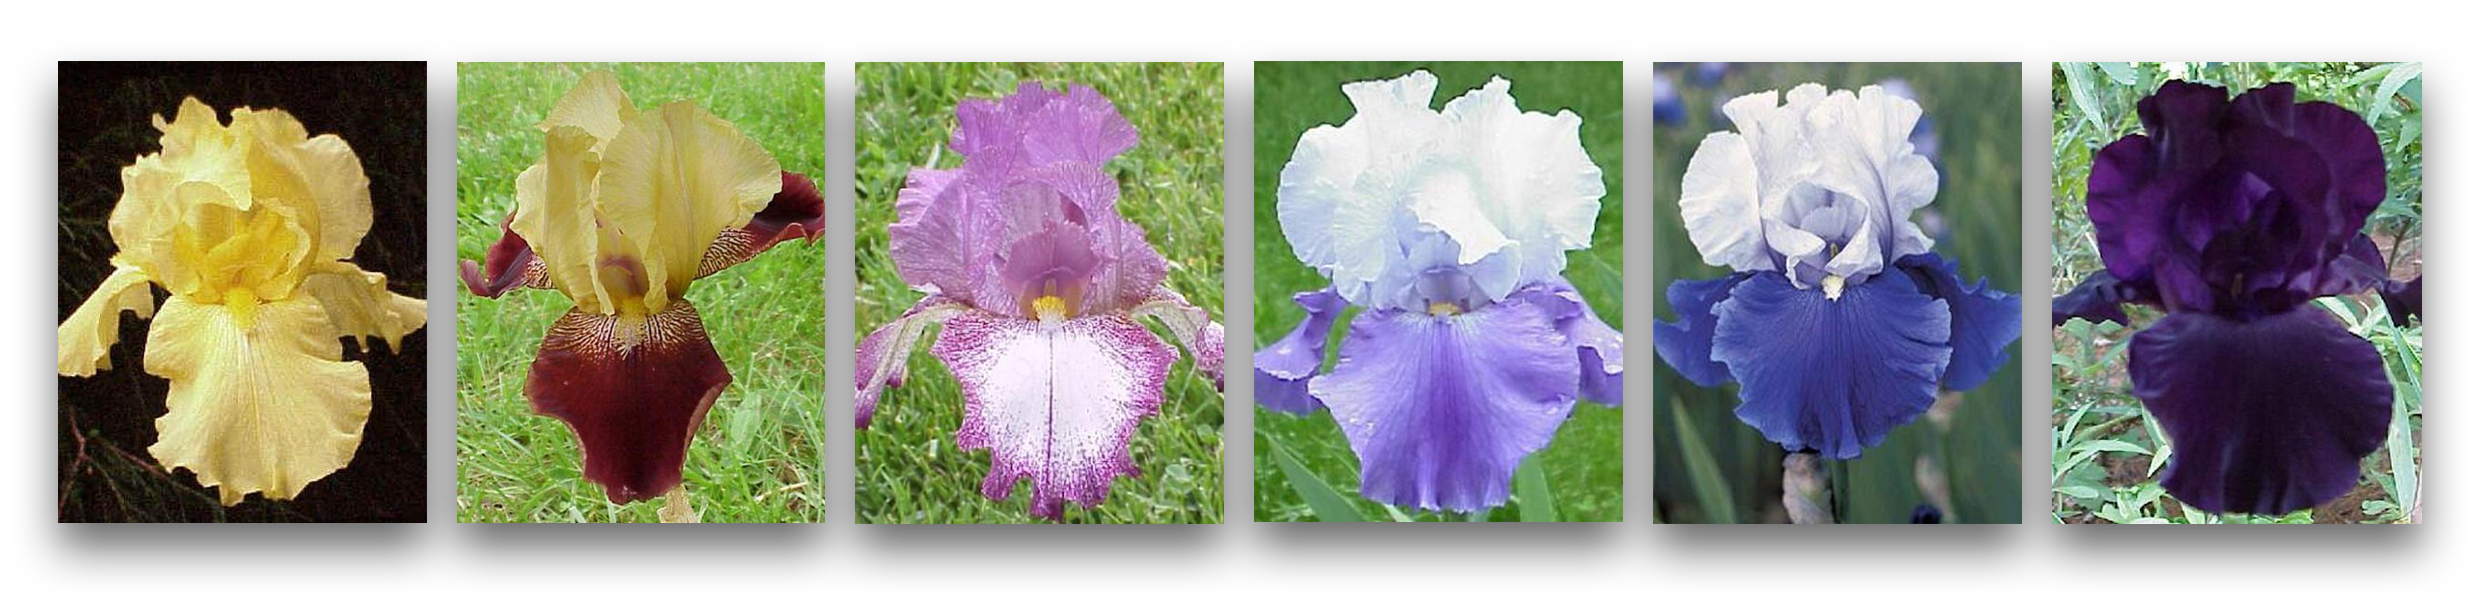
\includegraphics[totalheight=4cm]{img/37.png}
  \caption{Example images from category 6. Despite being of the same species, the flowers in the dataset differ visually}
  \label{img:37}
\end{figure}


%\textbf{Add analysis of 102 confusion matrix, neaten formatting of the diagrams over these few pages}
%TODO 102 flower analysis


\begin{figure}[hbt]
	\centering
  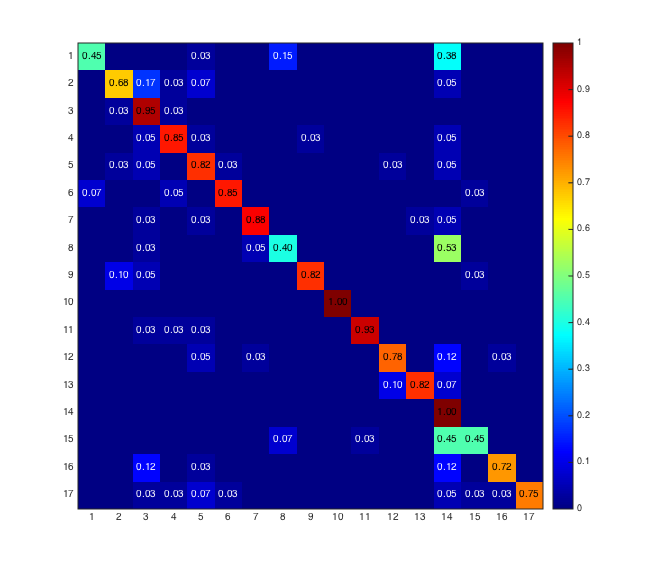
\includegraphics[totalheight=10cm]{img/31.png}
  \caption{Confusion matrix for the 17 flower dataset, obtained using mirroring and sampling}
  \label{img:31}
\end{figure}

\begin{figure}[hbt]
	\centering
  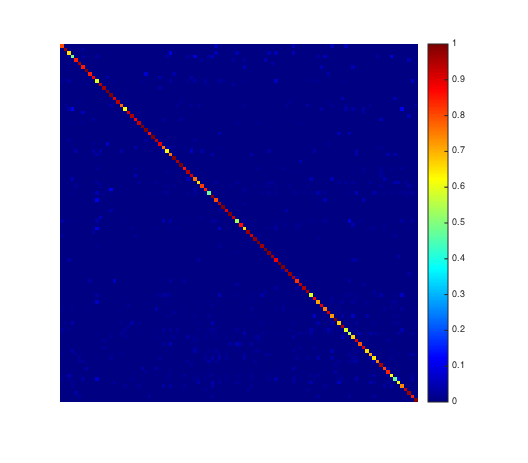
\includegraphics[totalheight=10cm]{img/32.png}
  \caption{Confusion matrix for the 102 flower dataset, obtained using mirroring and sampling}
  \label{img:32}
\end{figure}






\section{Training and test set augmentation}
\label{sec:augmentation}
%TODO introduce section

This section covers the techniques used to augment the training and test datasets. This is done as in some cases it has been shown to increase accuracy~\cite{Chatfield14}.

\subsection{Training set augmentation}
\label{sec:train_augmentation}

\begin{figure}[hbt]
	\centering
  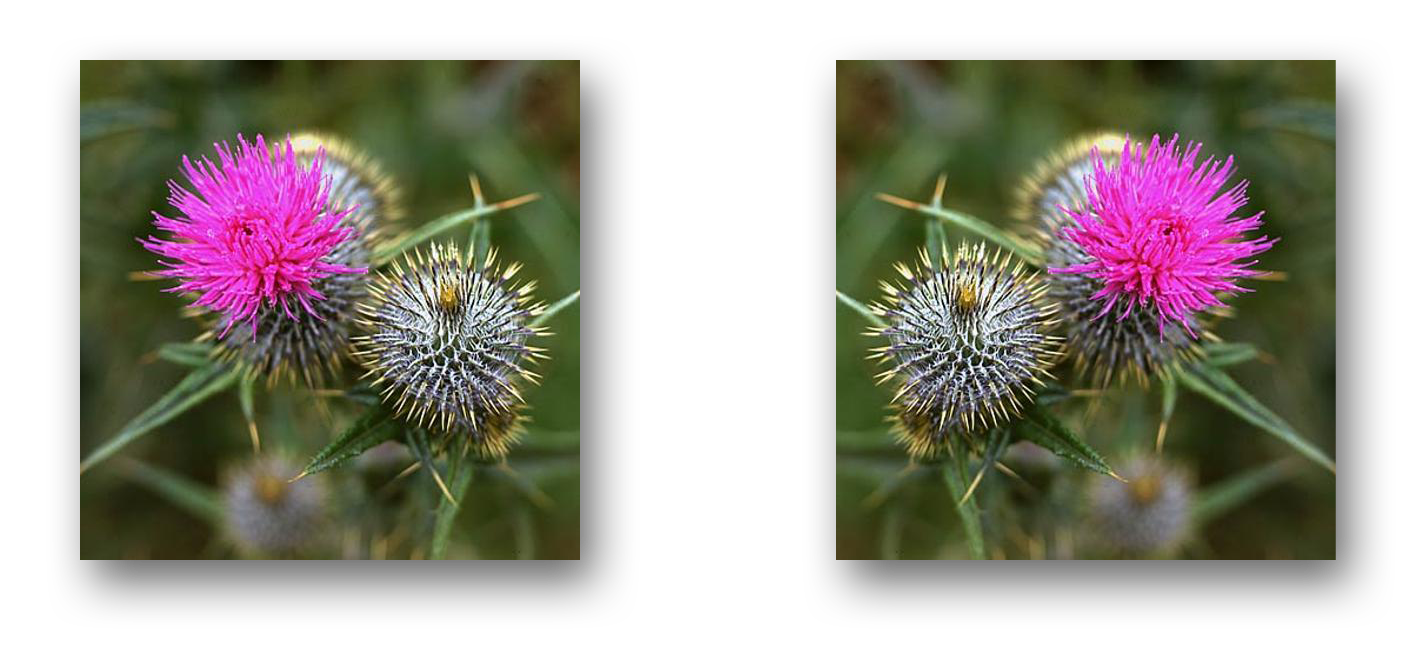
\includegraphics[totalheight=4cm]{img/09.png}
  \caption{An example flower shown with its vertical mirror}
  \label{img:09}
\end{figure}

\begin{figure}[hbt]
	\centering
  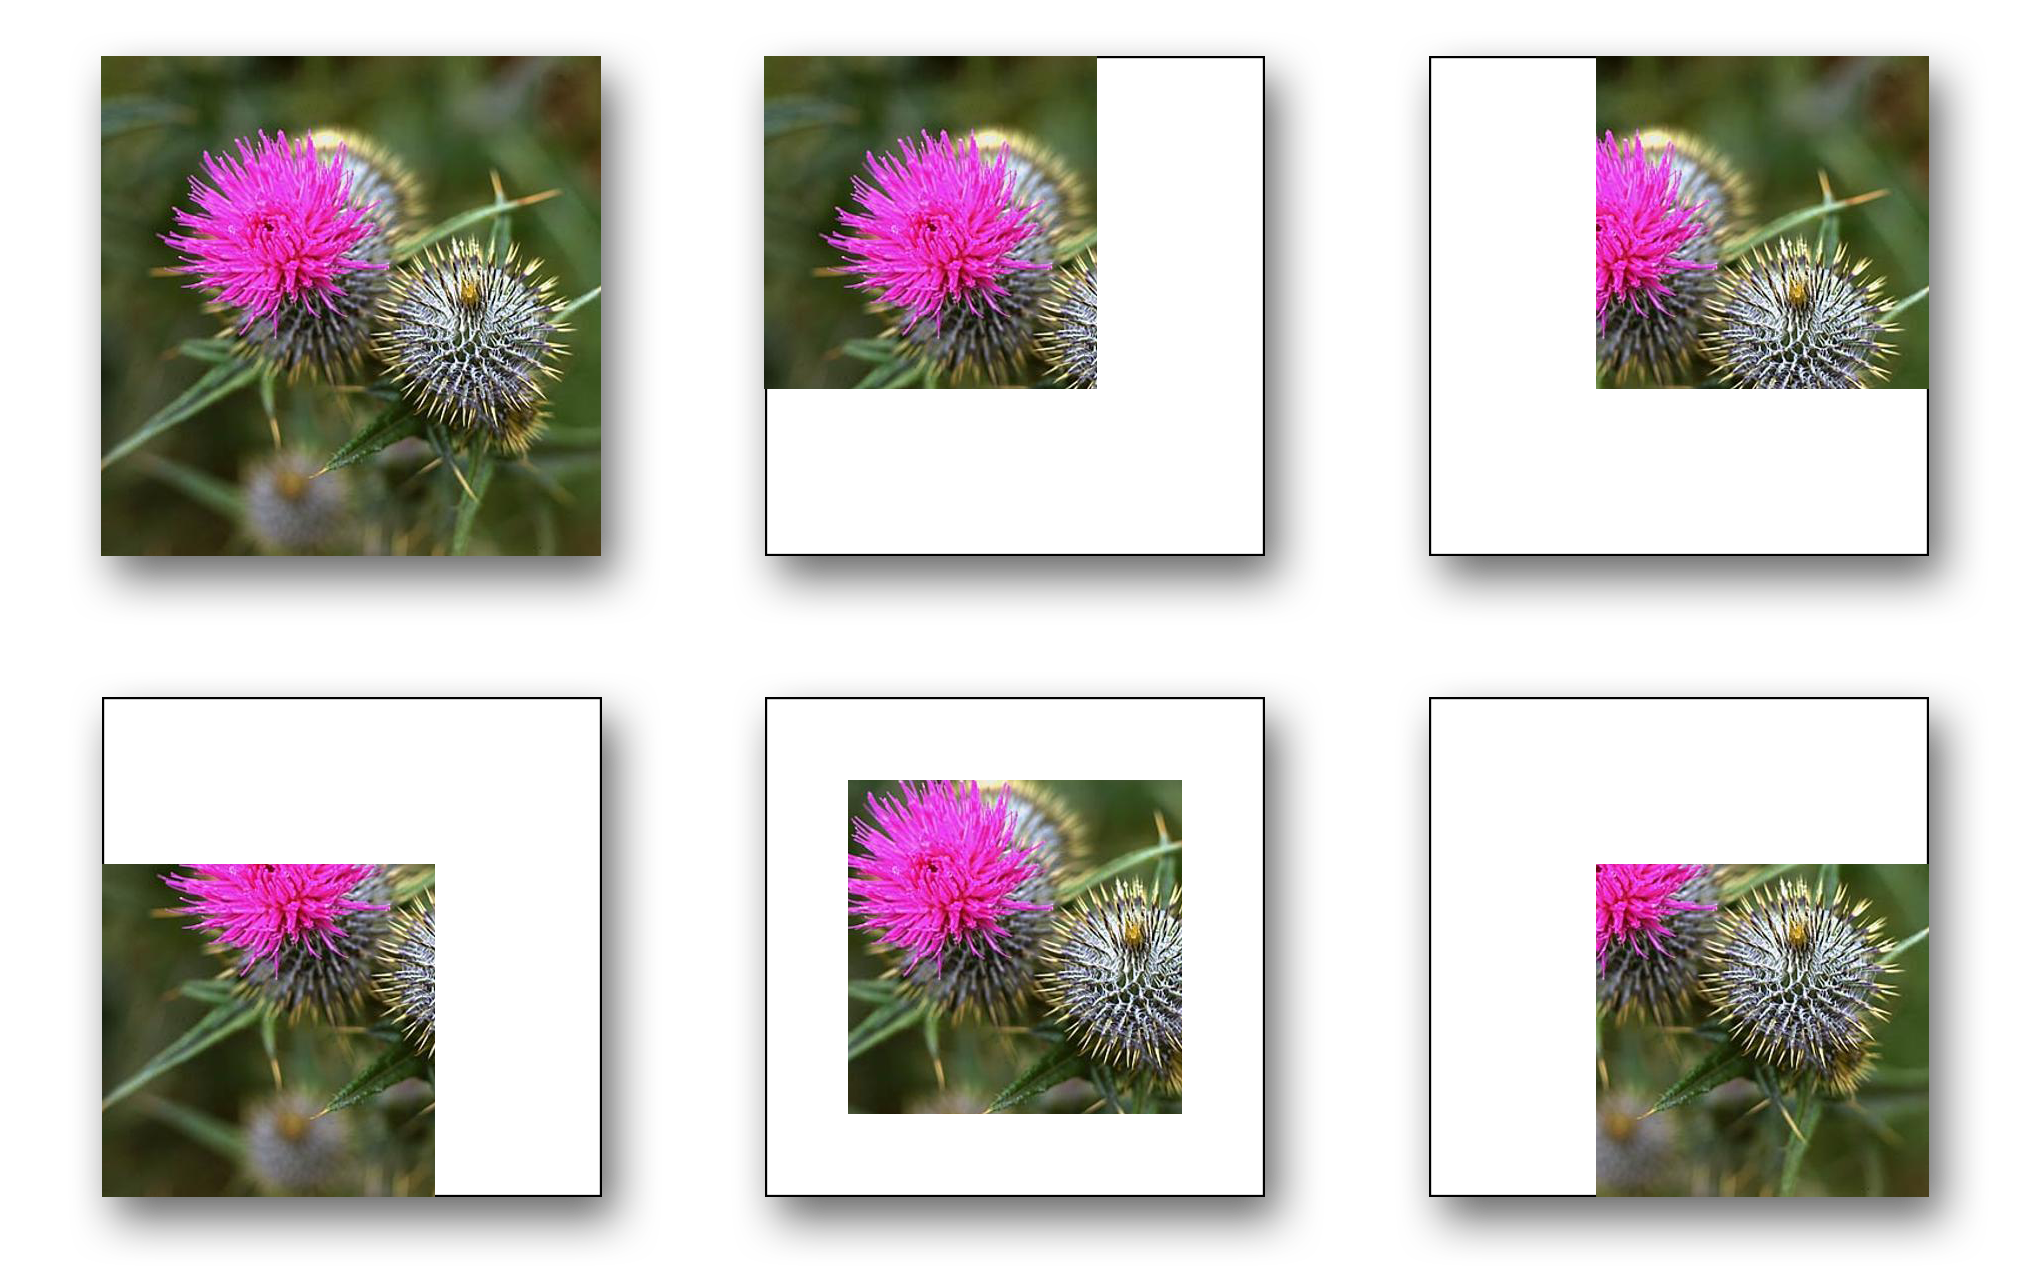
\includegraphics[totalheight=8cm]{img/10.png}
  \caption{An example flower shown with the images sampled from it}
  \label{img:10}
\end{figure}

Taking mirrors and samples of the images in the training set (Figures~\ref{img:09} and~\ref{img:10}) allows the training set to be expanded. The objective of this is to get the most out of the training set images. Both techniques generate new images from which new feature vectors can be calculated. These can be used to improve the quality of the SVM model. 

Only the vertical mirror can be used, as shown in Figure~\ref{img:09}, as flowers only exhibit vertical symmetry. 


\subsection{Test set augmentation}
\label{sec:test_augmentation}

For the same reasons as laid out above, mirroring and sampling the test image can improve classification accuracy.

For each image, several image vectors $\vect{x_{i}}$ are now being produced. Each one of these is run against the weight matrix to produce several vectors of prediction values $\vect{p_{i}}$. To classify the flower, these vectors of prediction values must be combined. This is done by finding the mean of each corresponding value.%, or by taking the maximum of each corresponding value:
$$
\begin{aligned}
	\vect{x} &= \frac{1}{n} \sum_{n = 0}^{n} \vect{x}_{i} \\
%	& or \\
%	&= max(\vect{x}_i)
\end{aligned}
$$







%-------------------------------
% Client and Server Architecture
%-------------------------------
\chapter{Client and server architecture}
\label{sec:client_server}

This chapter describes the implementation of the client and the server. It is concerned only with technical details, the look and feel of the application is discussed in the next chapter. The client is an application running on a user's Android phone. The application allows the user to send photo to the server over the internet. The server is a constantly running computer which runs the classification algorithms described in Section~\ref{sec:classification}. Upon receiving the photo, the server performs the classification and then returns the results to the application, where they are displayed. The server client architecture is shown in Figure~\ref{img:11}.


\begin{figure}[h]
	\centering
  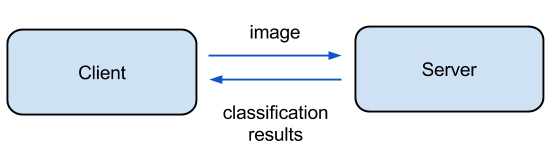
\includegraphics[totalheight=3cm]{img/11.png}
  \caption{Diagram showing the information flow between client and server}
  \label{img:11}
\end{figure}


\section{Client architecture} 

\begin{figure}[h]
	\centering
  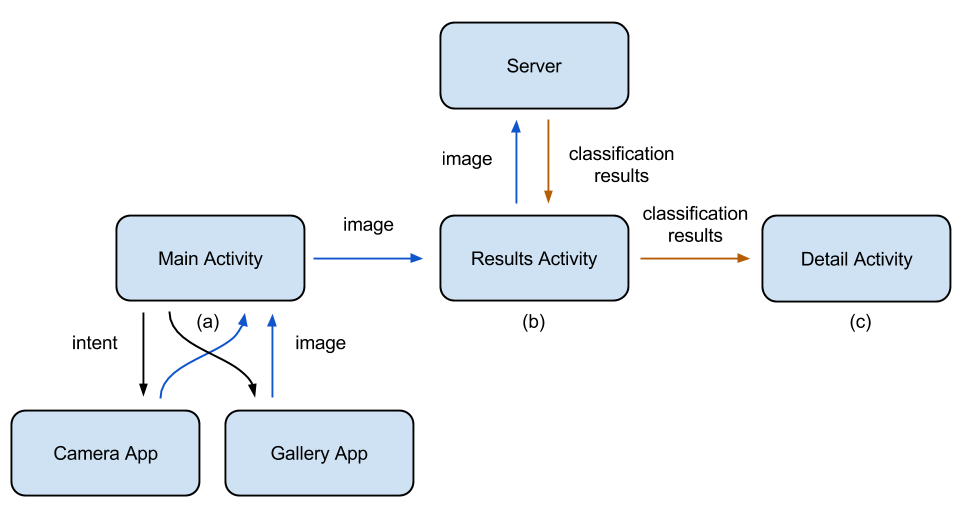
\includegraphics[totalheight=9cm]{img/12.png}
  \caption{Diagram showing the information flow between different sections of the client}
  \label{img:12}
\end{figure}

The client is an Android application made up of three activities\footnote{http://developer.android.com/reference/android/app/Activity.html}. Each activity is an object which allows the user to perform a specific task, and has a screen with which the user can interact with it. The functions of the activities are shown in Figure~\ref{img:12}. Screenshots of the activities are shown in Figures~\ref{img:47} and~\ref{img:39}.



\subsection{Taking the photo}

After the application is launched, the Main Activity of the application (Figure~\ref{img:12} (a)) presents the user with two buttons, which allow the user to take a photo, or upload a previously taken photo from a gallery. Both of these buttons trigger intent calls. Intents\footnote{http://developer.android.com/reference/android/content/Intent.html} are objects native to the Android system, which allow an application to request an action from another application component. The intent call starts the built-in camera or gallery application, and allows the user to take or choose a photo without having to write that code into the application. 

Once a photo is taken or chosen, the second activity of the application (Figure~\ref{img:12} (b)) is called, and the filename of the photo is passed to it. 


\subsection{Uploading the photo}

When the Results Activity (Figure~\ref{img:12} (b)) is called, a HTTP connection is opened, connecting to the URL of the server. A HTTP POST request is started, and the photo is uploaded to the server. The filename is appended to the POST request header as the value in a key-value pair. The key is predetermined and is used by the server to extract the image from the body of the request. 

The object which contains the code to upload the image extends a native Android object called an AsyncTask\footnote{http://developer.android.com/reference/android/os/AsyncTask.html}. The AsyncTask starts a new thread, and runs the upload code on it. This is done because the photo upload can take several seconds. If this were to take place on the user interface thread, user interface features such as scrolling and use of the navigation buttons could not take place until the uploading had been completed. This makes the application seem like it has frozen and is bad user experience design.

\subsection{Receiving results}

Once the photo has been uploaded to the server, and the classification has been carried out, the server responds with a JSON array containing the classification results and information about those flowers. 

The array consists of a number of flower objects, each of which contains the flower name, species, the URL of an example image, a snippet of information about the flower from Wikipedia and a links to that flower's Wikipedia page and google search.

The results are placed in a list, shown in Figure~\ref{img:39} (d, e), and the images are downloaded from their URLs using an image downloading and cacheing library named Picasso\footnote{http://square.github.io/picasso}. Picasso allows for the downloading, display and cacheing of an image with a single line of code. If the user scrolls down the list and an image scrolls off the screen, it is destroyed in order to save memory space. If the user scrolls up again, the cacheing implemented by Picasso allows that same image to be loaded from the cache, rather than be downloaded again. This improves performance as loading from memory is essentially instantaneous while downloading the image can take a few seconds.

If an image in the list is clicked, a detailed view of that flower is shown (Figure~\ref{img:39} (f, g, h)). This shows the user extra information about the flower, and presents them with buttons which allow them to Google search the flower or go to the flower's Wikipedia page. 



\section{Server architecture}


The server side consists of two servers, shown in Figure~\ref{img:07.png}. The first (front end) receives the image from the client, saves it to a folder and passes the filename to the second (back end) server. The second server calls a Matlab instance, and runs the Matlab classification script on the image. It constructs a JSON array of results and passes it to the first server which returns the results to the client. 

This two-server architecture improves security as file input and output is kept separate from the classification logic.

\begin{figure}[hbt]
	\centering
  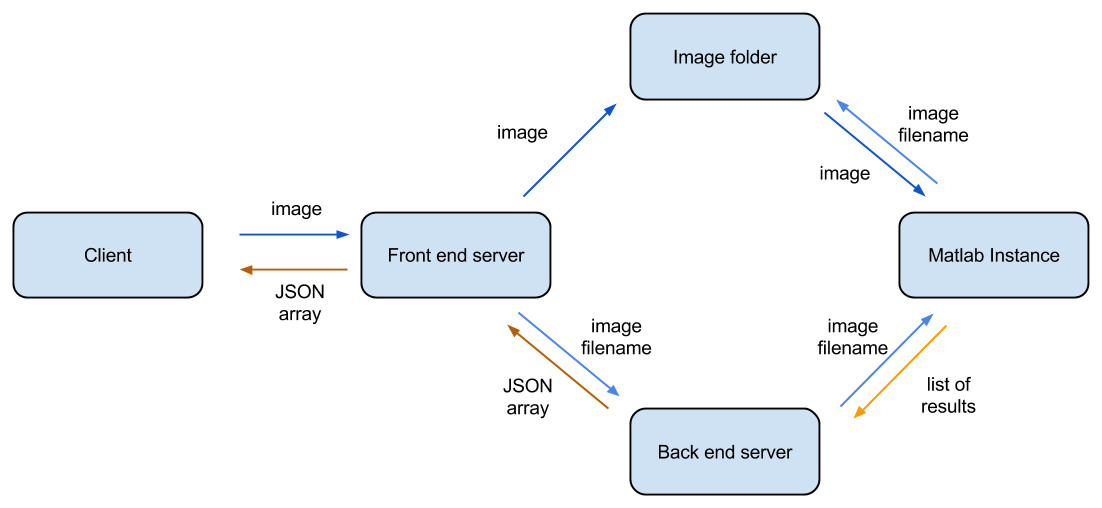
\includegraphics[totalheight=8cm]{img/07.png}
  \caption{Diagram showing information flow between the different sections of the server side}
  \label{img:07.png}
\end{figure}

\subsection{Flask server}

The front end server runs the Flask server framework\footnote{http://flask.pocoo.org/}. The server sets up a URL and checks it for incoming POST requests. When a POST request is detected, it checks the request header for the filename, using a predetermined key. It then uses the filename to download the image and saves it to the image folder. 

Error catching is implemented as the incoming POST requests cannot be assumed to necessarily be benevolent. The filetype is checked and only image files are downloaded. Flask's \verb|secure_filename| function is used to generate filenames for the images before they are saved. The secure filename function stops filenames which could negatively affect computer behaviour, and prevents name clashes.

% \subsection{Connection between servers}

\subsection{Backend server}

The backend server acts as a Python wrapper around the Matlab classification code. It uses the Python to Matlab bridge Mlwrap\footnote{http://mlabwrap.sourceforge.net/}, which allows Matlab functions as if they were Python functions. 


Upon starting, the server opens an instance of Matlab and loads the convolutional neural network and the weight matrix $\vect{W}$. Due to the large size of these files (245MB and 3.2MB respectively) loading takes several seconds but it only needs to be done once. By completing them upon start, they don't need to be run when a classification request is received, speeding up the classification time. 

It receives the filename from the front end server, and passes the filename and CNN to the Matlab classification function. This Matlab function returns a list of the category numbers of the eight top classification results. 

The backend server then constructs the JSON Array. Lists of flower names, species, image URL, Wikipedia text and Wikipedia and Google search URLs are stored. The appropriate information is chosen from the category numbers. This JSON array is passed back to the front end server which passes it to the client. 




%-------------------------------
% Application design
%-------------------------------
\chapter{Application design}
%"...describing the design of the app, showing screen shots of the interface as it goes through an example, plus a gallery of results."

This section covers the design of the application, the technical details of which were discussed in Chapter~\ref{sec:client_server}. The chapter is split into two sections: user interface and user experience. User interface considers how the application looks and how the user interacts with the application. User experience is concerned with the feel of the application; how fast, simple and intuitive it is to use. Screenshots of the application are given in Figure~\ref{img:39}.



\begin{figure}[h]
\centering
\begin{minipage}[b]{0.2\linewidth}
	\centering
	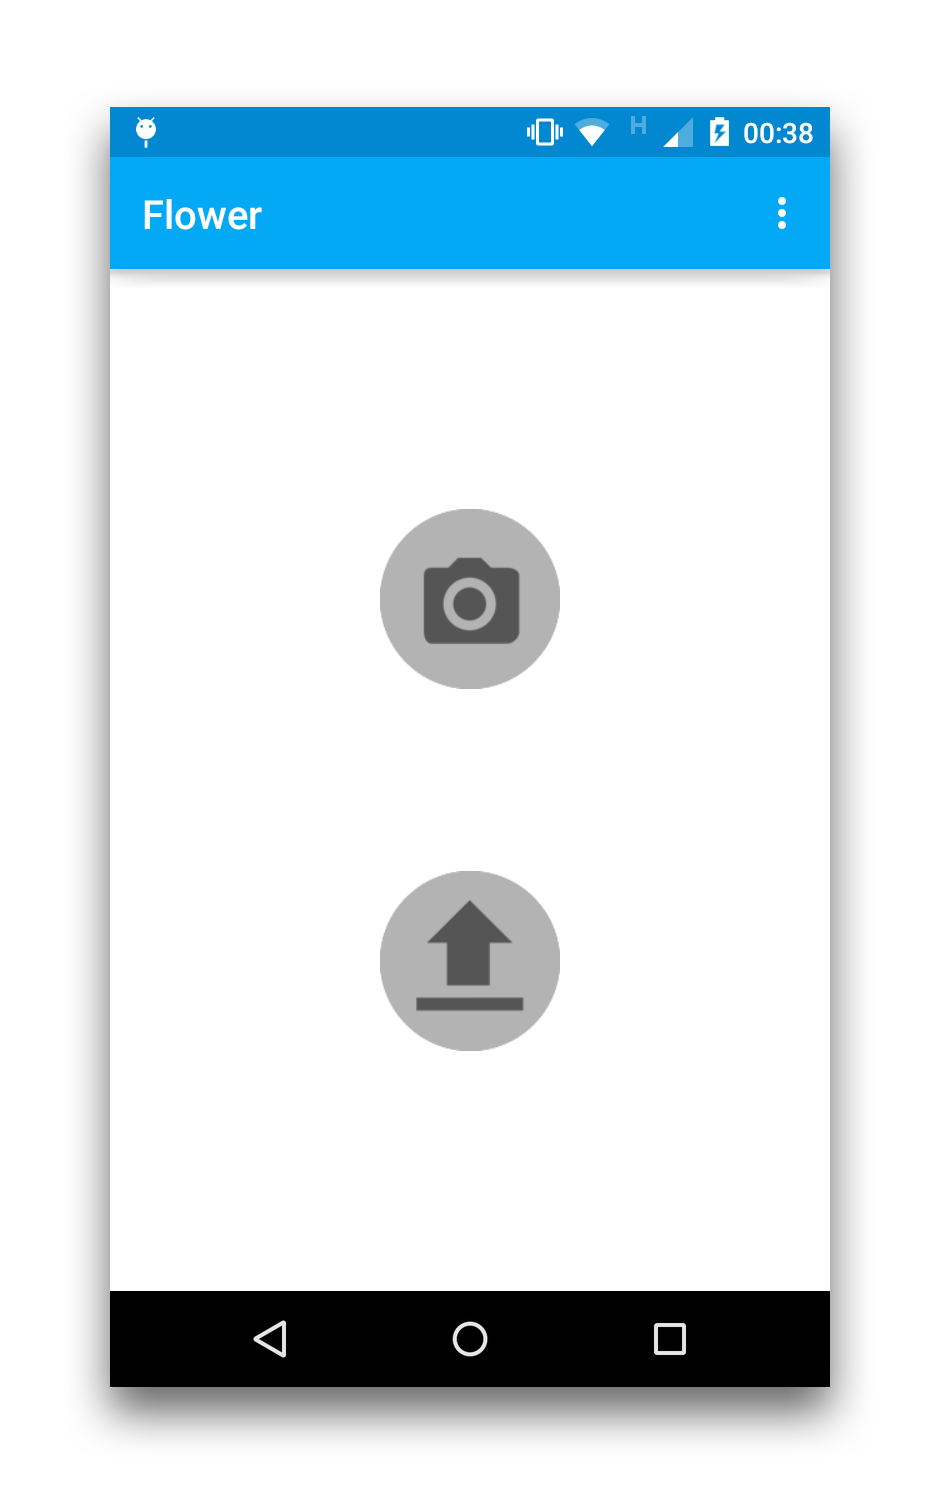
\includegraphics[totalheight=6cm]{img/39.png}
	(a)
\end{minipage}
\begin{minipage}[b]{0.2\linewidth}
	\centering
	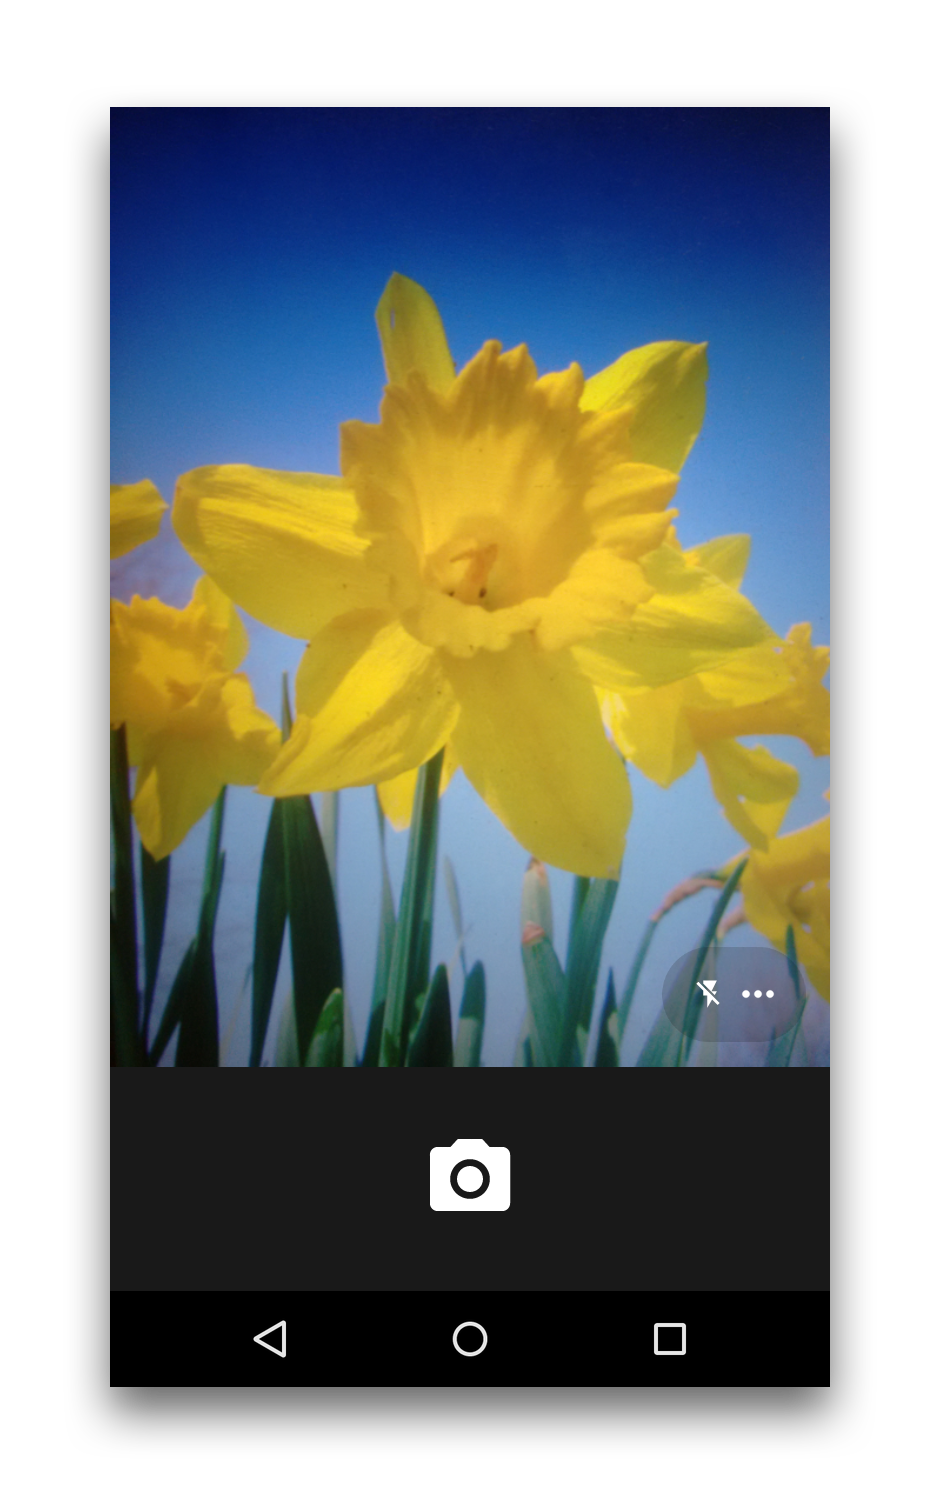
\includegraphics[totalheight=6cm]{img/40.png}
	(b)
\end{minipage}
\begin{minipage}[b]{0.2\linewidth}
	\centering
	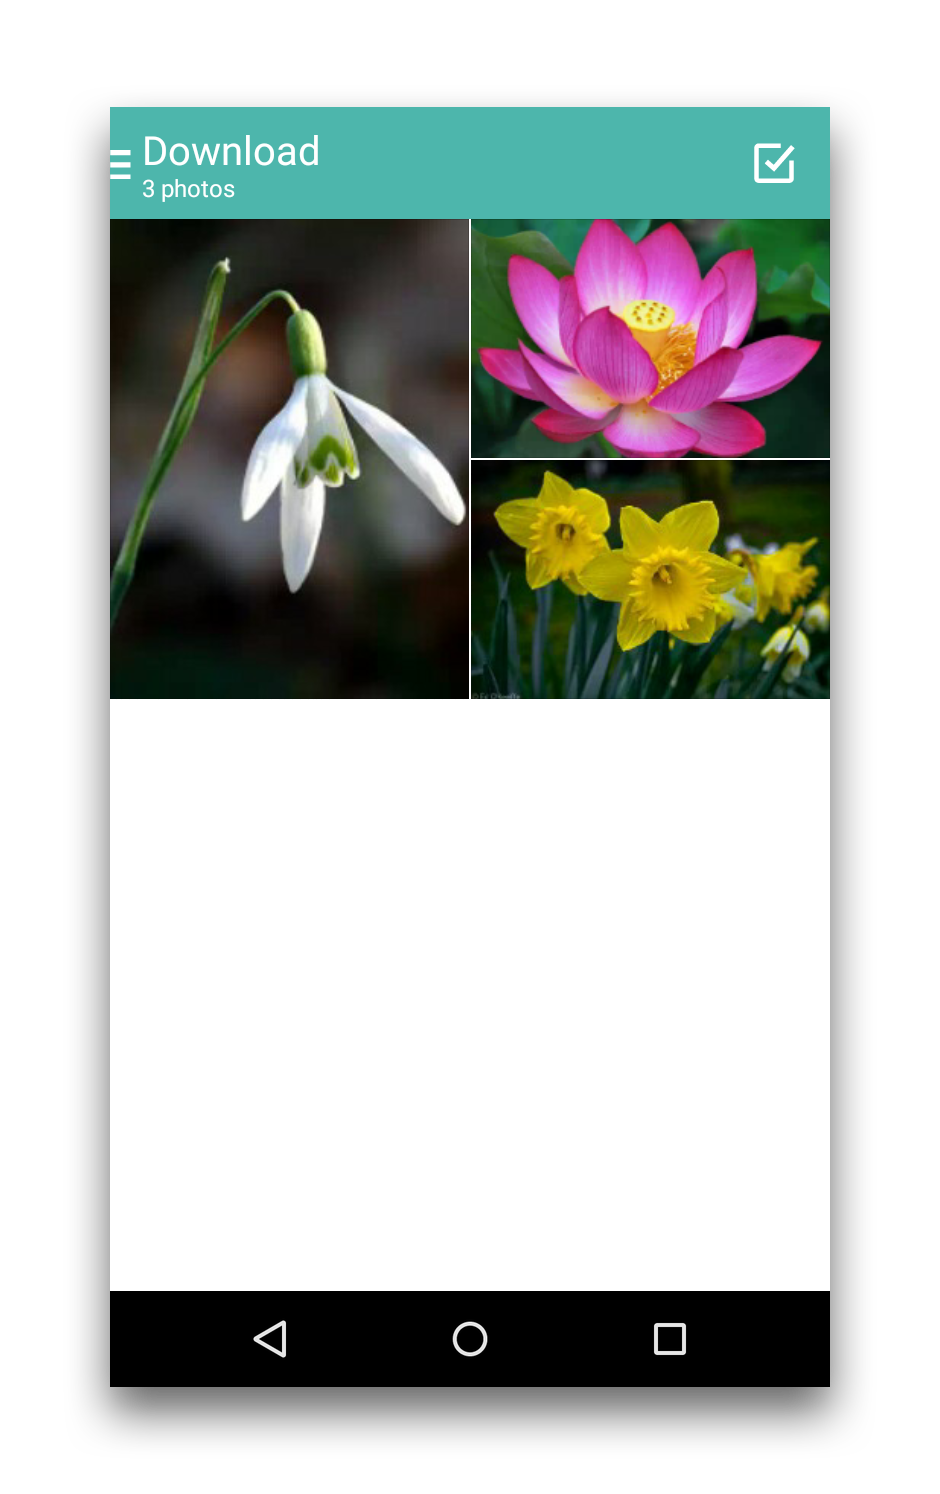
\includegraphics[totalheight=6cm]{img/41.png}
	(c)
\end{minipage}
\begin{minipage}[b]{0.2\linewidth}
	\centering
	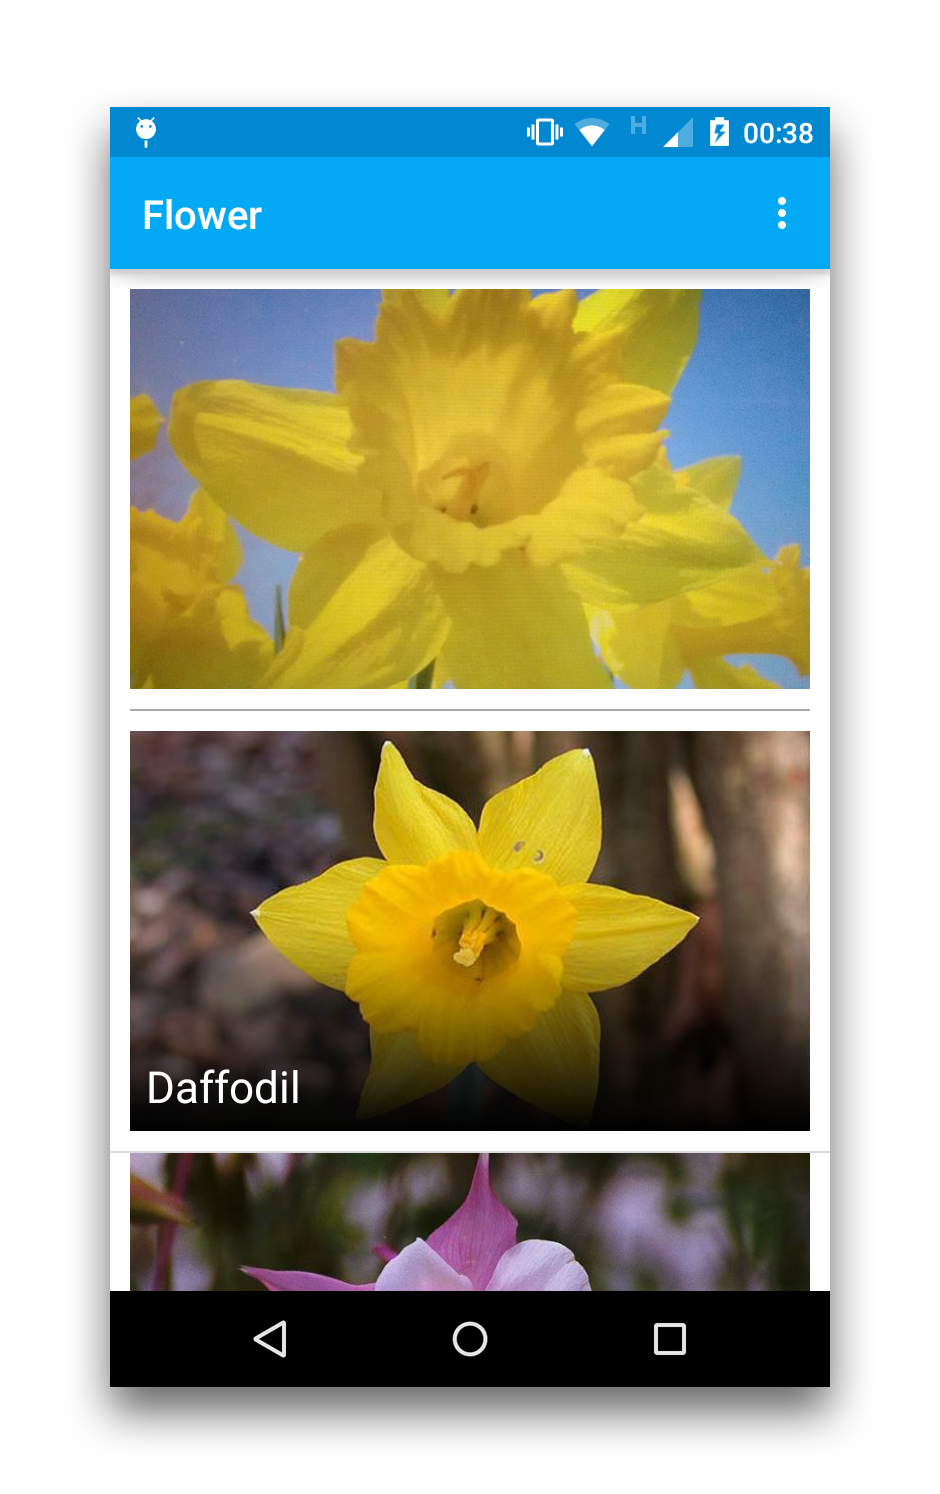
\includegraphics[totalheight=6cm]{img/42.png}
	(d)
\end{minipage}
\begin{minipage}[b]{0.2\linewidth}
	\centering
	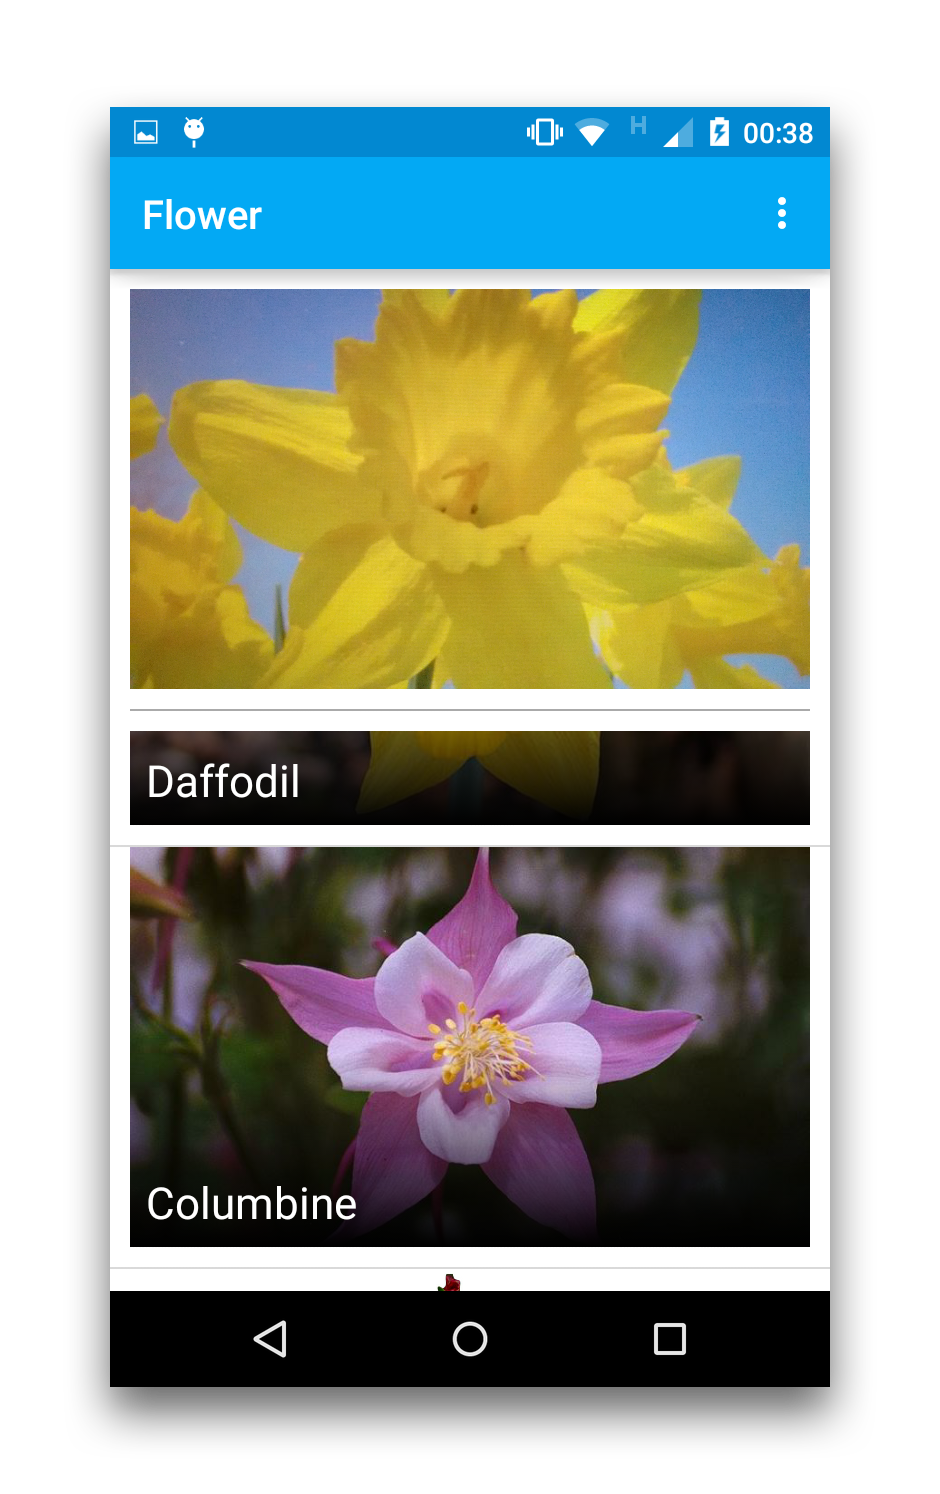
\includegraphics[totalheight=6cm]{img/43.png}
	(e)
\end{minipage}
\begin{minipage}[b]{0.2\linewidth}
	\centering
	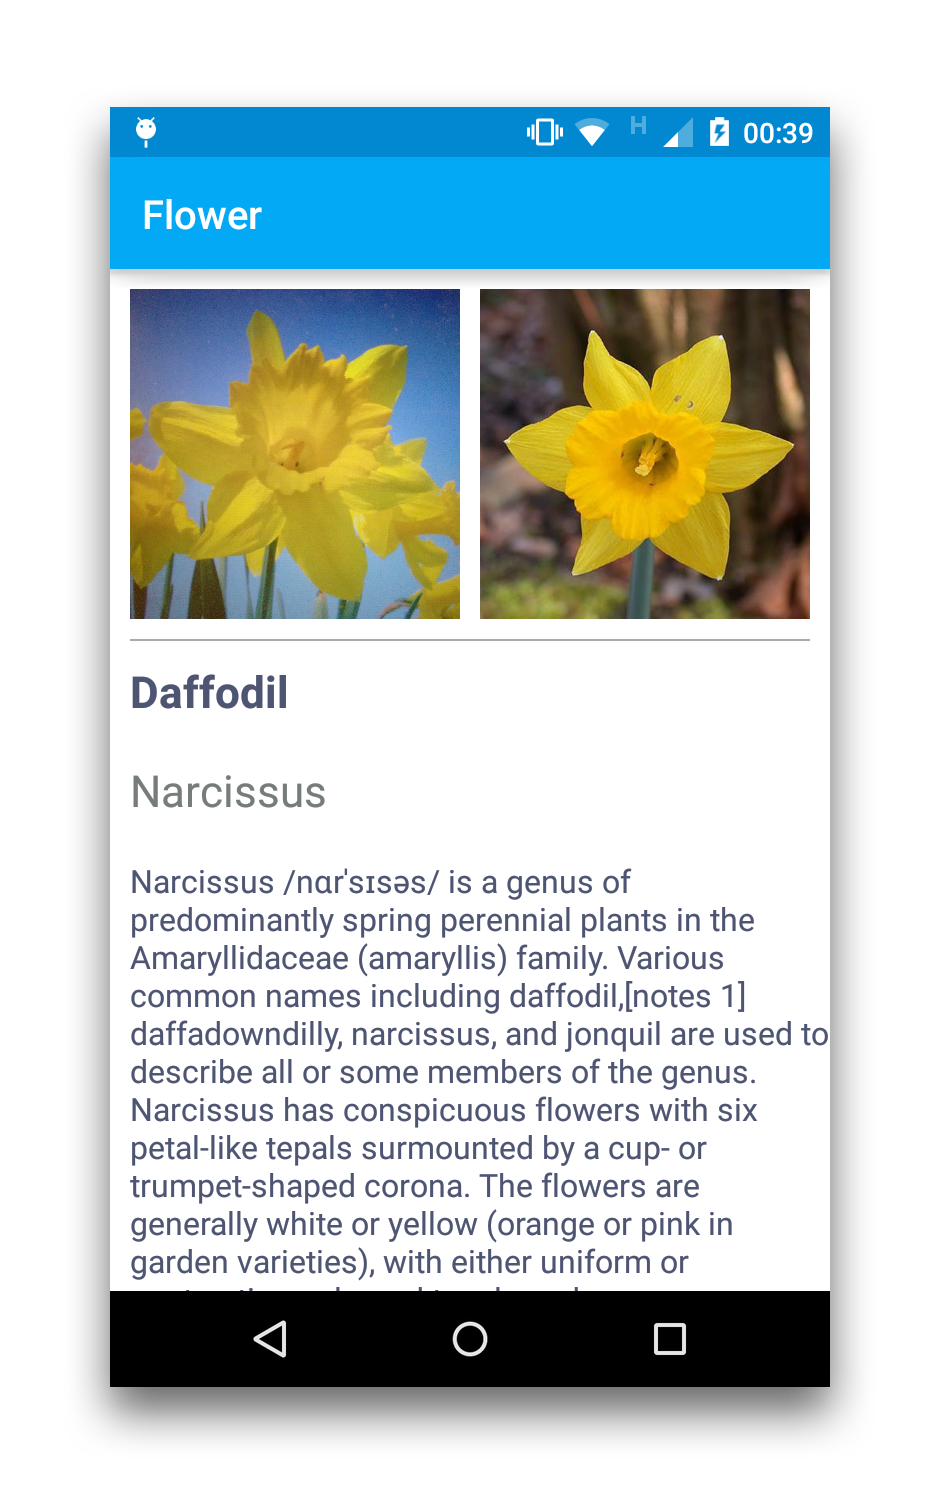
\includegraphics[totalheight=6cm]{img/44.png}
	(f)
\end{minipage}
\begin{minipage}[b]{0.2\linewidth}
	\centering
	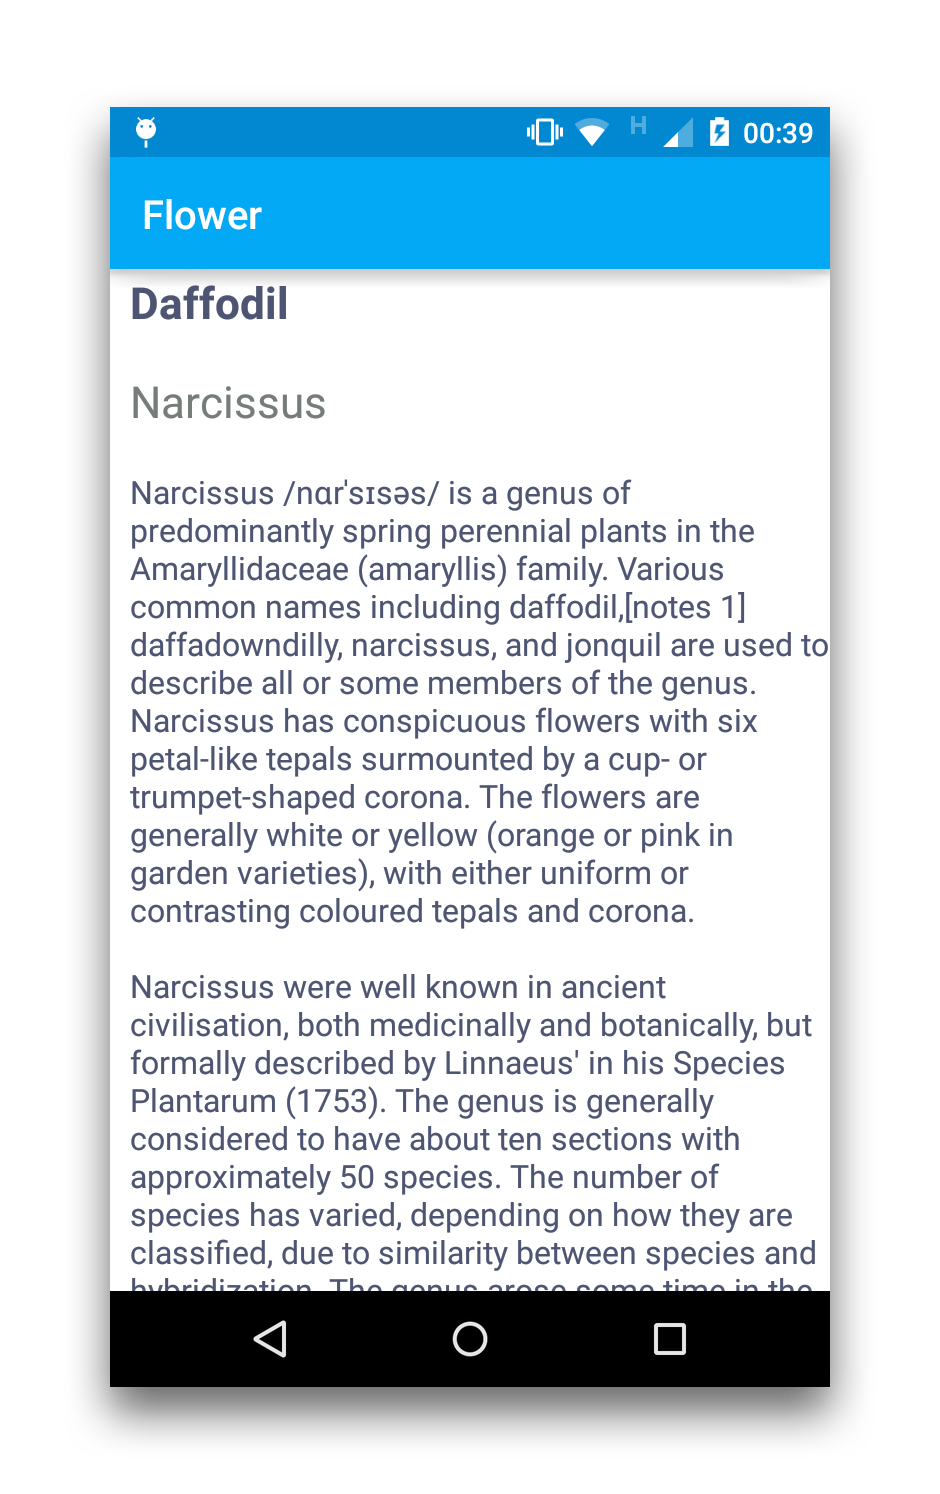
\includegraphics[totalheight=6cm]{img/45.png}
	(g)
\end{minipage}
\begin{minipage}[b]{0.2\linewidth}
	\centering
	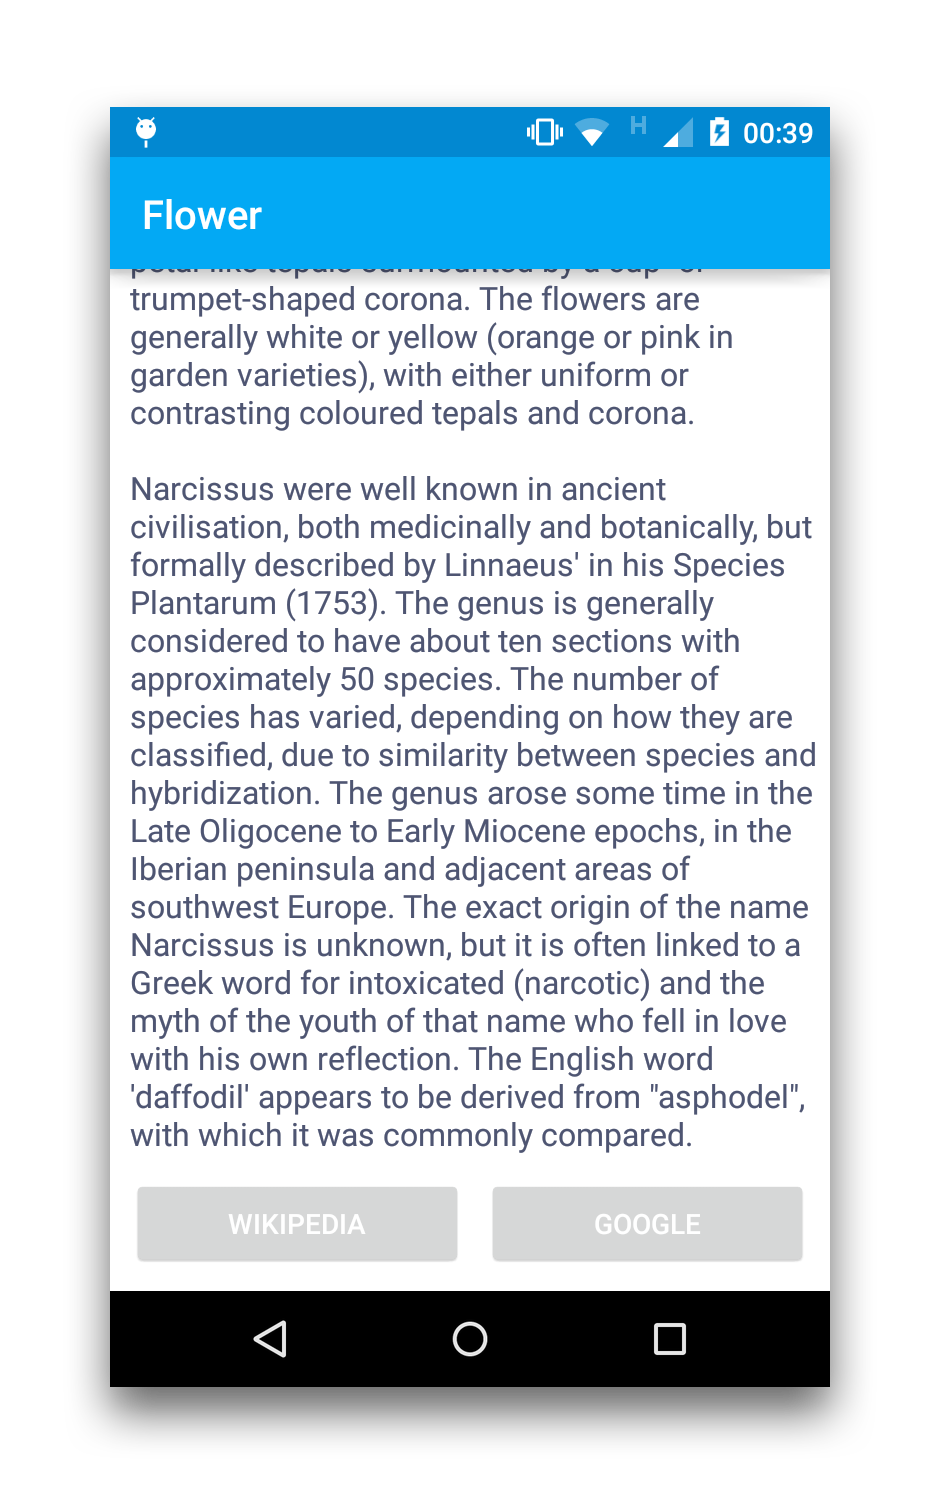
\includegraphics[totalheight=6cm]{img/46.png}
	(h)
\end{minipage}

\caption{Screenshots of the application. (a): The Main Activity allows the user to choose whether to take or upload a photo. (b, c): The user takes a photo or chooses one to upload. (d, e): Results Activity. The photo is uploaded, classified and the results are displayed in a scrollable list. (f, g, h): Detail Activity. If one of the images in (d,e) is clicked, a detail view of that flower is shown.}
\label{img:39}
\end{figure}




\section{User interface design}

The user interface has been optimised by following Android's design guidelines\footnote{https://developer.android.com/design/index.html}. This results in an Application which looks and behaves like applications the user has seen before, making it familiar and intuitive to use. 

\subsection{Material theme}

The application implements Android's recently released Material theme\footnote{https://developer.android.com/design/material/index.html}. Material is the latest design standard released by Google. It introduces shadows, animations and code snippets which allow easy implementation of new features. Some examples of applications running the Material theme are shown in Figure~\ref{img:38}. The Material theme is used to keep the application familiar to Android users. 

\begin{figure}[hbt]
	\centering
  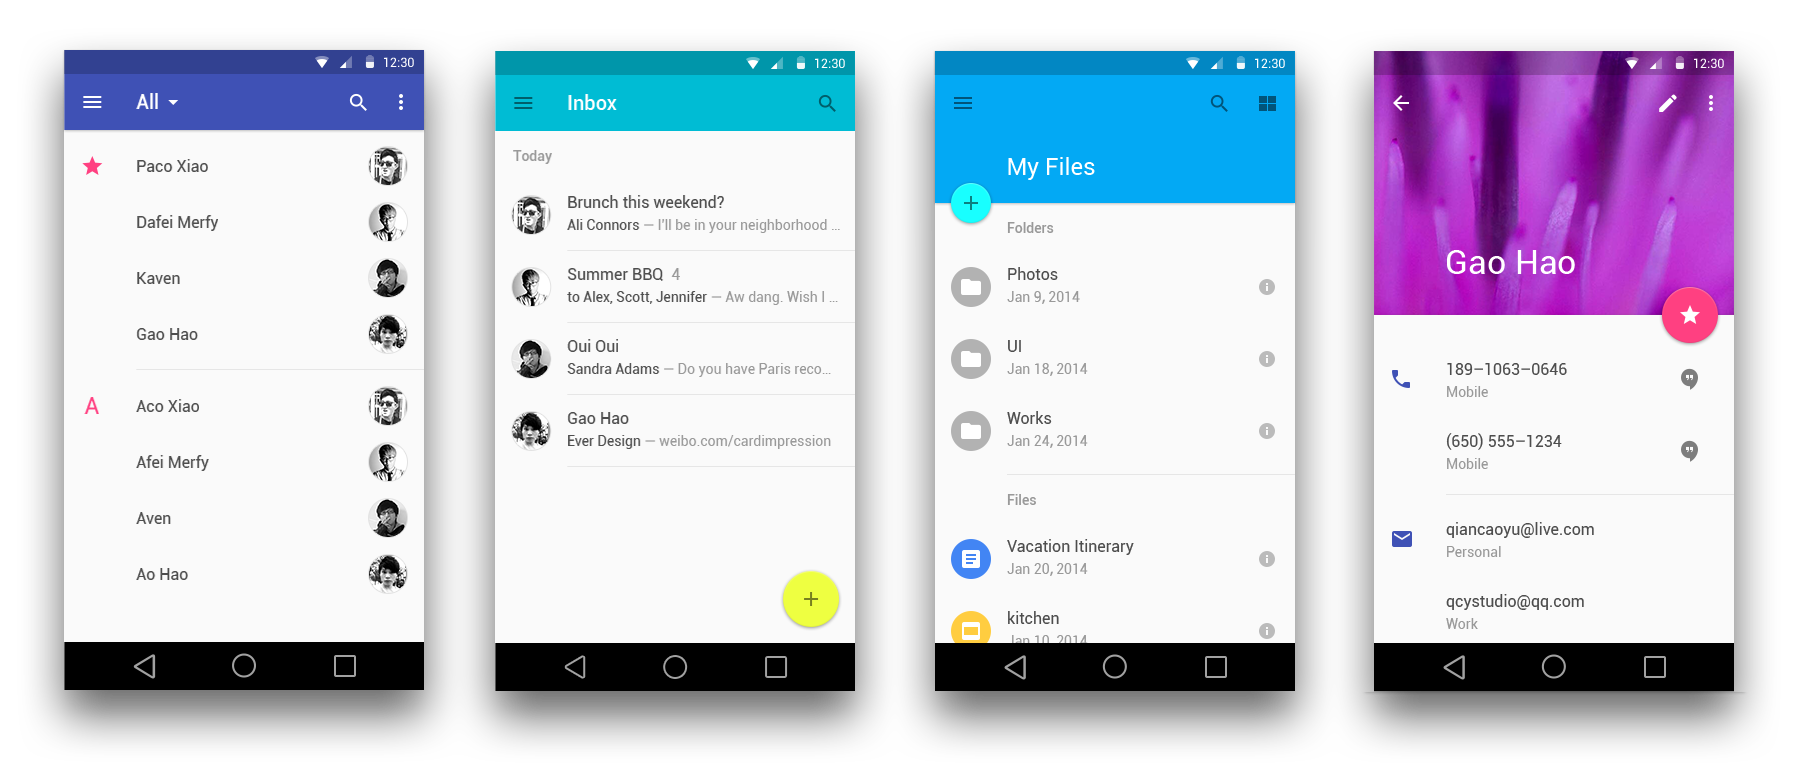
\includegraphics[totalheight=7cm]{img/38.png}
  \caption{Examples of applications using the Android Material theme}
  \label{img:38}
\end{figure}

 While the full Material theme can only run on devices running the latest version of Android, version 5.0 (API level 21), the look of the theme can be replicated on older devices by using Android's \verb|AppCompat| theme. 


\subsection{List and detail views}

The results of the classification are presented in a list (Figure~\ref{img:39} (d, e)), showing an image of the flower and the flower's common name. Above the list the photo the user has taken is shown, allowing for easy comparison. The images are cropped such that they are large enough to show the flower without taking up too much screen space. Each item on the list is clickable, and clicking reveals a page which details more information about that flower (Figure~\ref{img:39} (f, g, h)). This is a common way of presenting data and will be familiar to most users.


\subsection{Button design}

\begin{figure}[hbt]
	\centering
  
\includegraphics[totalheight=3cm]{img/13.png}
  \caption{The unpressed and pressed versions of the Take Photo and Upload Photo buttons}
  \label{img:13}
\end{figure}

The take photo and upload photo buttons are custom designed (Figure~\ref{img:13}), and use icons rather than words for simplicity. The icons used are adapted from the official Android icon pack\footnote{https://developer.android.com/design/downloads/index.html\#action-bar-icon-pack}, and will be familiar to Android users. The buttons use flat colour, keeping with the Material theme. Both pressed and unpressed buttons have been made, and the change in colour gives visual feedback to the user that the button has been pressed. 

\section{User experience design}

User experience has been optimised by focusing on making the classification as fast as possible and the application as simple to use as possible. 

\subsection{Simplification}

By keeping the application simple, it is easier to use. The application presents the user with a single choice; whether to take a photo or to upload a photo which has been previously taken. Uploading and downloading happens automatically, and no menu options are provided except the ability to share the result of a classification. 

\subsection{Flower images}

\begin{figure}[hbt]
	\centering
  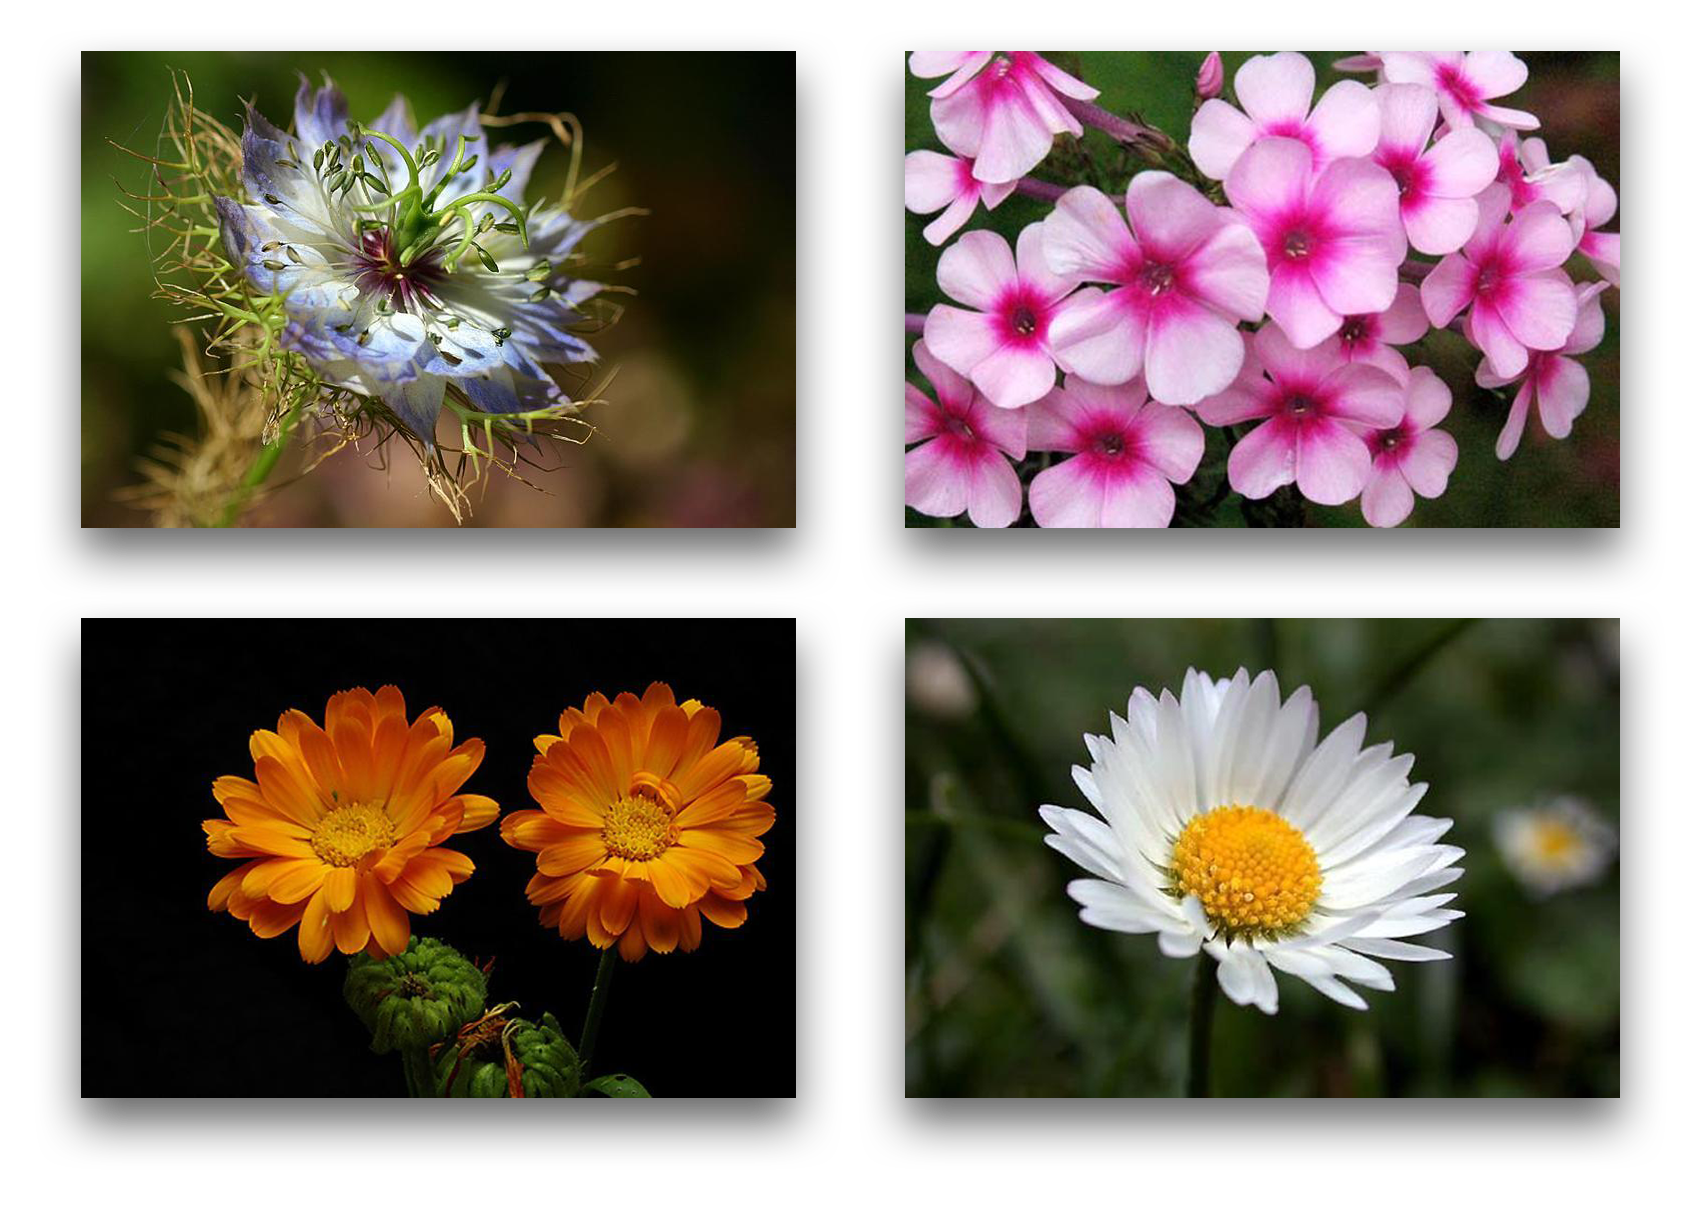
\includegraphics[totalheight=8cm]{img/14.png}
  \caption{A selection of the hand-picked flower images shown to the user}
  \label{img:14}
\end{figure}

After classification takes place, a ranked list of the six most likely flower species is passed to the client and the user. An algorithm was written which finds the flower image in the dataset most similar to the photo uploaded by the user for each of the six species.  %Similarity is found by finding $min|x - y_i|$
%TODO fix this equation



Similarity is found by finding the smallest difference $min|y_i - x|$ between the uploaded flower's feature vector $x$ and the feature vector $y_i$ for all $i$ photos in the dataset. 

Although this improves ease of use, this process also greatly increases classification time, as the image must be compared to each image in six categories, where the number of images in each category is up to 258. It also requires a copy of the feature vectors of all the images in the 102 dataset to be stored, which takes up 39MB of storage space. This slight increase in ease of use is not worth the increases in classification time and server footprint.

Instead of this, 102 example flowers have been hand-picked for their quality. They have been chosen because they all clearly display the flower in question whilst minimising any confusing background. The images are cropped to the dimensions they will be displayed at, minimising the amount of data which needs to be transferred and speeding up the downloading time. 




\chapter{Summary and future work}
% Mirror of intro. Intro discusses challenges, conclusions describe how challenges were minimised. Were goals achieved


\section{Summary}

This project applied modern computer vision techniques to the problem of flower species classification. The scope of the problem was limited to the 102 flower species laid out in the Oxford 102 category flower dataset. An accuracy of 85.6\%, and a rank accuracy of 96.2\% when considering the top six ranks was obtained. 

A mobile application was designed and created with intuitiveness, simplicity and speed in mind. The classification pipeline was made accessible from the application, allowing free quick and accurate flower classification from anywhere in the world with an internet connection.

\section{Future work}

\subsection{Expand flower species covered}

The application currently classifies 102 flower species, and it should be a priority to expand this number as users will expect the application to work for a larger set of flowers. This could be done by obtaining a list of all common flower species in a certain geographical location, for example the UK, and then finding enough images of each of those species to train an SVM classifier. The images could be found by contacting horticultural bodies who have access to such images, or by searching online image repositories such as Google Images or Flickr. More images for each category will increase the accuracy of the models. However, this project has obtained an effective accuracy of 96.2\% using only 20 training images per species. 

\subsection{No good classification option}

It would appear unpolished if the application gave normal classification results for an image which is not a flower. An additional step to the classification pipeline could be added which notifies the user if the image is not considered to be of a flower. Even if this is the case, the normal classification results would still be provided, in case the photo is in fact of a flower. 

This could be implemented in two ways. A loose-grained classification step could be added. This would check whether the image is indeed a flower, before the image is passed to the fine-grained classification. Implementing this would require training another one-vs-the-rest SVM classifier which is trained on all of the flower images marked as belonging to the flower category, and images of other common items marked as belonging to the 'rest' category. These other images would have to be found. At runtime, this extra classification step requires a single dot product to be calculated and will not add much to the total classification time, and if the SVM model is trained well it should accurately distinguish between photos of, and not of, flowers. 

It could also be implemented by giving a warning if highest prediction value $p_i$ was below some threshold value $T$, indicating that there was low similarity between the models user's image. This is easy to implement, as only a few lines of code would have to be added, although a suitable $T$ would have to be found. This and adds very little to the classification time, however it may not be as accurate as the above method. 

\subsection{Storing flower data on phone}
\label{sec:data_on_phone}

Flower data such as common names, species and images could be hard written into the application. After classification, rather than sending all data associated with the classification predictions, a simple list of identification number could be sent, from which the application constructs the list presented to the user. This would reduce classification time slightly as less data would have to be downloaded, but would increase the size of the application by around 8MB, most of which is used to store the images. 


\subsection{Porting CNN to phone}

All of the classification pipeline could easily be written into the application code with the exception of the convolutional neural network. The CNN consists of layers written in C++, connected together with Matlab code. Matlab code cannot easily be compiled down to code runnable in an Android environment, so porting the CNN to Android would involve rewriting the Matlab code in C or C++, and then compiling that to Android runnable code using the Android NDK\footnote{http://developer.android.com/tools/sdk/ndk/index.html}. 

Porting the CNN to the phone would allow for complete offline classification, if the flower data were also stored on the phone, as described in~\ref{sec:data_on_phone}. The effect it would have on total classification depends on several factors. Uploading and downloading time is completely removed, but as the phone has less processing power than the server, the actual classification may take longer. Whether this improves classification time will depend on a user's individual circumstances, such as the quality of their internet connection and the power of their phone.


\subsection{Database of flowers}

The flower information, Wikipedia text and images are currently stored in lists at the index of the appropriate category. A more scalable system would be to refactor the code to use a database with an entry for each flower, indexed with a unique ID. Each entry stores the flower information, Wikipedia text, weight vector and image associated with it. When booting, a weight matrix could be generated using all available weight vectors. While this would not change functionality, it would allow for new flowers to be added with greater ease.

\subsection{iPhone app}

Finally, an iPhone version of this application could be written. This would take the form of a client application which takes a photo, uploads it to the same server which has already been created and then receives and displays the results. 




%-------------------------------
% Bibliography
%-------------------------------
\printbibliography

\end{document}
